\documentclass[aip,jcp,reprint,noshowkeys,superscriptaddress]{revtex4-1}
\usepackage{graphicx,dcolumn,bm,xcolor,microtype,multirow,amscd,amsmath,amssymb,amsfonts,physics,longtable,wrapfig}
\usepackage[version=4]{mhchem}

\usepackage[utf8]{inputenc}
\usepackage[T1]{fontenc}
\usepackage{txfonts}

\usepackage[
    colorlinks,
    linkcolor={red!50!black},
    citecolor={red!70!black},
    urlcolor={red!80!black}
	]{hyperref}
\urlstyle{same}

\DeclareUnicodeCharacter{0308}{\"{}}


\newcommand{\ie}{\textit{i.e.}}
\newcommand{\eg}{\textit{e.g.}}
\newcommand{\alert}[1]{\textcolor{red}{#1}}
\usepackage[normalem]{ulem}
\usepackage{tikz}
\usetikzlibrary{decorations.markings,decorations.pathreplacing,arrows.meta}
\newcommand{\titou}[1]{\textcolor{red}{#1}}
\newcommand{\trashPFL}[1]{\textcolor{\red}{\sout{#1}}}
\newcommand{\PFL}[1]{\titou{(\underline{\bf PFL}: #1)}}

\newcommand{\cre}[1]{\Hat{a}_{#1}^{\dag}}
\newcommand{\ani}[1]{\Hat{a}_{#1}}
\newcommand{\ca}[2]{\Hat{a}^{#1}_{#2}}

\newcommand{\mc}{\multicolumn}
\newcommand{\fnm}{\footnotemark}
\newcommand{\fnt}{\footnotetext}
\newcommand{\tabc}[1]{\multicolumn{1}{c}{#1}}
\newcommand{\QP}{\textsc{quantum package}}
\newcommand{\T}[1]{#1^{\intercal}}

% coordinates
\newcommand{\br}{\boldsymbol{r}}
\newcommand{\bx}{\boldsymbol{x}}
\newcommand{\bI}{\boldsymbol{1}}
\newcommand{\cK}{\mathcal{K}}

% orbital energies
\newcommand{\eps}{\epsilon}
\newcommand{\irr}{\text{irr}}

% shortcuts for greek letters
\newcommand{\si}{\sigma}
\newcommand{\la}{\lambda}
\newcommand{\ii}{\mathrm{i}}
\newcommand{\up}{\uparrow}
\newcommand{\dw}{\downarrow}
\newcommand{\upup}{\up\up}
\newcommand{\updw}{\up\dw}
\newcommand{\dwup}{\dw\up}
\newcommand{\dwdw}{\dw\downarrow}

\newcommand{\h}{\text{1h}}
\newcommand{\p}{\text{1p}}
\newcommand{\hp}{\text{1h+1p}}
\newcommand{\hhp}{\text{2h1p}}
\newcommand{\pph}{\text{2p1h}}
\newcommand{\ph}{\text{ph}}
\newcommand{\eh}{\text{eh}}
\newcommand{\he}{\text{he}}
\newcommand{\ee}{\text{ee}}
\newcommand{\teh}{\overline{\text{eh}}}
\newcommand{\pp}{\text{pp}}
\newcommand{\hh}{\text{hh}}
\newcommand{\xc}{\text{xc}}
\newcommand{\Hx}{\text{Hx}}

% addresses
\newcommand{\LCPQ}{Laboratoire de Chimie et Physique Quantiques (UMR 5626), Universit\'e de Toulouse, CNRS, UPS, France}

\begin{document}

\title{From the three-particle Green's function to the parquet equations,
to ADC, and beyond}

\begin{abstract}
In three stages, these notes point out the connection between the parquet and the ADC
constructions of the self-energy. First, we show that the
single-particle Green's function is naturally
expressed in terms of the three-particle Green's
function through the Martin--Schwinger hierarchies of
equations of motion for $n$-th order Green's functions.
We then introduce the Faddeev decomposition of the 
three-particle vertex and show that it naturally leads to 
the parquet approximation of the self-energy. 
In a next step, finite-order Faddeev kernels are introduced, 
and it is shown, for $n=1,2$ that the formalism with the 
$n$th-order Faddeev kernel, before any resummation, 
is equivalent to GF($n+2$). Within the Tamm--Dancoff approximation (TDA) 
to the $\eh$ and $\pp$ Bethe--Salpeter equations, 
ADC(3)/ADC(4) are obtained. Beyond the TDA, 
to first order in the Faddeev kernel we obtain a
Hermitian version of the Faddeev random-phase approximation (FRPA), and at fourth order 
we obtain a new partial parquet approximation. 
Full parquet is significantly more involved, and includes 
a) an internally resummed infinite-order Faddeev kernel, 
b) cross-channel interactions, and c) self-consistency in the 
single-particle propagator. 
\end{abstract}

\maketitle
\tableofcontents

\section{Introduction}
\label{sec:introduction}
Via the three-particle Green's function $G_3$,
two routes to the one-particle self-energy are connected: the
parquet equations for the two-particle vertex and the
algebraic-diagrammatic construction (ADC).
Starting from the
Martin--Schwinger hierarchy (Sec.~\ref{sec:MS}), we express the
correlation self-energy in terms of a 6-point response function $R$,
which is obtained from $G_3$ by subtracting a one-particle reducible
part and which obeys a Dyson equation with a three-particle kernel
(Sec.~\ref{sec:eliminating}).

By dropping the 3-body irreducible kernel, 
the three-particle kernel is approximated by its Faddeev part,
\cite{Faddeev1961,Winter1972,Ethofer1969} that 
describes scattering of two of the three lines 
through a two-particle vertex, while the third line is a spectator.
The two-particle vertex that lets these lines interact pairwise
is the full parquet vertex $F$.\cite{Kugler2018}
The resulting self-energy contains the Neumann series
of the Faddeev kernel, whose resummation induces couplings between
the parquet vertices in all channels.
Truncating the Faddeev kernel at order $m$ ($m=1,2$) and keeping all
terms of the Neumann series up to the same total order, the GF($m+2$)
self-energy is obtained, and the diagrammatic matching of Schirmer
gives ADC($m+2$). ADC(3) needs only the linear term with the
first-order kernel, while ADC(4) also needs the product of two
first-order kernels.
This is merely a laborious way to
derive ADC. ADC(3) is worked out as an
illustrative case in App.~\ref{app:ADC}. ADC(4) follows equally.
ADC(5) does not follow from the third-order Faddeev kernel, since the
3-body irreducible kernel contributes at fifth order.

The connection becomes more useful once the vertices in the pairs are
resummed beyond the Tamm--Dancoff ladders contained in ADC
(Sec.~\ref{sec:parquet_Heff}). Within
the parquet approximation and with a Hartree--Fock reference, all
interactions are instantaneous, and the usual 
time-ordering rules turn the
Faddeev series into resolvents of configuration spaces.
In this way, with the full RPA ladders of the first-order Faddeev
kernel in every pair,
a Hermitian effective Hamiltonian of the size of ADC(3) is obtained
that describes the coupling of a single particle to
particle-particle ($\pp$) and electron-hole ($\eh$) phonons.
This is essentially the Faddeev random-phase approximation (FRPA) of
Barbieri and
co-workers.\cite{Barbieri2001,
barbieri2003extension,
barbieri2007quasiparticles,
Degroote2011}
In the
Tamm--Dancoff approximation of the phonons, the FRPA matrix reduces to
the ADC(3) matrix, while its couplings reduce to $U^{(1)}$.
In contrast to parquet, FRPA
contains neither the crossed channels inside a pair, nor the
overlapping time-orderings of different pairs. The hierarchy is
$
\text{ADC(3)}
\subset
\text{FRPA}
\subset
\text{parquet}
$ for the dynamic self-energy.

In coupled-cluster language, the ground-state correlations of the FRPA
phonons are three independently solved sets of channel amplitudes:
ring-CCD for the $\eh$ pairs and ladder-CCD for the $\pp$
pair.\cite{Scuseria2013} Full CCD couples these channels through its
crossed-ring and mosaic terms.\cite{Shepherd2014} 
These play the role of the crossed channels of parquet, but the precise
correspondence between the channel crossings in both approaches
remains to be discovered.

\begin{table}[hbt!]
\caption{Order through which the self-energy is exact, and the highest
ADC($n$) contained, for different approximations. $\Lambda$: fully
irreducible two-particle vertex; $K_{\rm 3B}$: 3-body irreducible
kernel; SDE: Schwinger--Dyson equation. The second row is the
construction of these notes. The first three rows use the parquet
approximation,
$\Lambda=\Lambda^{(1)}$, Eq.~\eqref{eq:crossing_Lambda}.}
\label{tab:orders}
\begin{ruledtabular}
\begin{tabular}{lccc}
Approximation & Eqs. & exact through & contains \\
\hline
Parquet, SDE
& \eqref{eq:SDE_G2}, \eqref{eq:parquet_BSE} & 4th & ADC(4) \\
Parquet $F$, Faddeev
& \eqref{eq:Faddeev_rearr}, \eqref{eq:Faddeev_F} & 4th & ADC(4) \\
Parquet $F$ $+$ $K_{\rm 3B}^{(3)}$
& \eqref{eq:R}, \eqref{eq:Sigma_closed} & 5th & ADC(5) \\
$\Lambda^{(\le4)}$, SDE
& \eqref{eq:SDE_G2}, \eqref{eq:parquet_BSE} & 5th & ADC(5) \\
$\Lambda^{(\le4)}$ $+$ $K_{\rm 3B}^{(\le4)}$
& \eqref{eq:R}, \eqref{eq:Sigma_closed} & 6th & ADC(6) \\
\end{tabular}
\end{ruledtabular}
\end{table}

Analogously, with the second-order Faddeev kernel, ADC(4) is obtained,
and with RPA ladders a fourth-order variant of FRPA. No
construction of these notes is exact beyond fourth order in the
self-energy. At fifth order, they all become approximate.
In the Schwinger--Dyson equation, the vertex
enters the self-energy with one explicit interaction, so that the
self-energy through order $n$ needs the fully irreducible vertex
$\Lambda$ through order $n-1$. Since $\Lambda$ has no 
second- and third-order contributions, the parquet approximation gives the
self-energy exactly through order $n=4$.
In the three-particle route taken here,
$R$ enters with two explicit interactions, so that the self-energy
through order $n$ needs the three-particle kernel through order $n-2$.
At $n=5$, the three-particle kernel is needed to third order. Since
its 3-body irreducible part has been dropped, the Faddeev route does
not give the self-energy exactly through order $n=5$.

The resulting orders are collected in Table~\ref{tab:orders}.
The step from
ADC(4) to ADC(5) requires the lowest-order 3-body irreducible
kernel. An improved $\Lambda$ does not help; it
becomes necessary only for ADC(6).
Since the diagrams that $\Lambda^{(n-1)}$
supplies to the self-energy at order $n$ in the Schwinger--Dyson route
must be supplied by the 3-body kernel at order $n-2$ in the
three-particle route, we expect both routes to lack the same diagrams at a given
order.


\section{Martin--Schwinger Equations}
\label{sec:MS}
Let us define the $n$-particle Green's function as 
\begin{equation}
	\label{eq:Gn_definition}
\begin{aligned}
G_n(1\ldots n;1'\ldots n')
={}&
(-\ii)^n
\big\langle
\mathcal{T}_{\mathcal{C}}\,
\hat{\psi}(1)\cdots\hat{\psi}(n)
\\
&\times
\hat{\psi}^{\dagger}(n')\cdots\hat{\psi}^{\dagger}(1')
\big\rangle \;,
\end{aligned}
\end{equation}
with $\hat{\psi}$ in the Heisenberg picture.
$G_n$ might be expressed in terms of $G_{n-1}$ and
$G_{n+1}$ through the
Martin--Schwinger hierarchy,
\begin{align}
&
\left[
\ii\partial_{t_1}
-
h_0(1)
\right]
G_n(1\ldots n;1'\ldots n')
\nonumber\\
={}&
\sum_{j=1}^{n}
(-1)^{j-1}
\delta(1j')\,
G_{n-1}
\bigl(
2\ldots n;
1'\ldots \widehat{j'}\ldots n'
\bigr)
\nonumber\\
&+
(-1)^{n}\,\ii\,
v(1\bar2;\bar3\bar4)\,
G_{n+1}
\bigl(
\bar3\bar4\,2\ldots n;
1'\ldots n'\bar2^{+}
\bigr) \;.
\label{eq:Martin_Schwinger_general}
\end{align}
We define 
\begin{equation}
G_0^{-1}(11')
=
\left[
\ii\frac{\partial}{\partial t_1}
-
h_0(1)
\right]
\delta(11') \;,
\label{eq:G0_inverse_def}
\end{equation}
and its inverse via
\begin{equation}
\label{eq:G0_inverse}
G_0^{-1}(1\bar{1})\,
G_0(\bar{1}1')
=
\delta(11') \;.
\end{equation}
Using both relations, $G_1$ through $G_4$
become
\begin{align}
G(11')
= & 
G_0(11')
\nonumber\\
& -\ii \,
G_0(1\bar3)\,
v(\bar3\bar4;\bar5\bar6)\,
G_2(\bar5\bar6;1'\bar4^+) \;,
\label{eq:Martin_Schwinger_G1} \\
G_2(12;1'2')
= & 
G_0(11')G(22')
-
G_0(12')G(21')
\nonumber\\
& +
\ii \,
G_0(1\bar3)\,
v(\bar3\bar4;\bar5\bar6)
\nonumber\\
&\times
G_3(2\bar5\bar6;1'2'\bar4^+) \;,
\label{eq:Martin_Schwinger_G2}\\
G_3(123;1'2'3')
= &
G_0(11')\,
G_2(23;2'3') \nonumber \\
& -
G_0(12')\,
G_2(23;1'3')
\nonumber\\
& +
G_0(13')\,
G_2(23;1'2')
\nonumber\\
& -
\ii\,
G_0(1\bar4)\,
v(\bar4\bar5;\bar6\bar7)
\nonumber\\
&\times
G_4(23\bar6\bar7;1'2'3'\bar5^+) \;,
\label{eq:Martin_Schwinger_G3}
\\
G_4(1234;1'2'3'4')
=&
G_0(11')\,
G_3(234;2'3'4') \nonumber \\
& -
G_0(12')\,
G_3(234;1'3'4')
\nonumber \\
& +
G_0(13')\,
G_3(234;1'2'4') \nonumber \\
& -
G_0(14')\,
G_3(234;1'2'3')
\nonumber\\
& +
\ii\,
G_0(1\bar5)\,
v(\bar5\bar6;\bar7\bar8) \nonumber  \\
& \times G_5(234\bar7\bar8;1'2'3'4'\bar6^+).
\label{eq:Martin_Schwinger_G4}
\end{align}
Through Eq.~\eqref{eq:Martin_Schwinger_G1}, we can define the single-particle
self-energy according to 
\begin{equation}
	\Sigma(11')
	=
	-\ii
	v(1\bar2;\bar3'\bar2')
	G_2(\bar3'\bar2';\bar3\bar2^+)
	G^{-1}(\bar3 1') \;.
	\label{eq:SDE_G2}
\end{equation}
\section{Eliminating $G_2$}
\label{sec:eliminating}
We can now use Eq.~\eqref{eq:Martin_Schwinger_G2}
to eliminate the dependence of 
Eq.~\eqref{eq:SDE_G2} in favour of $G_3$. 
Using Eq.~\eqref{eq:Martin_Schwinger_G3} 
and Eq.~\eqref{eq:Martin_Schwinger_G4}, 
one can see that $G_4$ might be eliminated as well, 
and Eq.~\eqref{eq:SDE_G2} can be expressed in terms 
of $G_3$ and $G_5$, or, more generally, in terms 
of odd-order Green's functions. Alternatively,
combining
Eq.~\eqref{eq:Martin_Schwinger_G2} with 
Eq.~\eqref{eq:Martin_Schwinger_G3}, one can express 
Eq.~\eqref{eq:SDE_G2} in terms of $G_2$ and $G_4$,
or, more generally, in terms 
of even-order Green's functions.

Here, we take the odd-order route. To do so, following 
\citet{Winter1972} and \citet{Ethofer1969}, 
we introduce the 6-point response function
\begin{equation}
\begin{split}
    R(123;1'2'3')
    &=
    G_3(123;1'2'3')
    \\
    &\quad
    -
    G_2(23;3'\bar4)\,
    G^{-1}(\bar4\bar4')\,
    G_2(\bar4'1;1'2') \;,
\end{split}
\label{eq:response_function}
\end{equation}
so that the EOM for $G_2$ becomes
\begin{align}
G_2(12;1'2')
&=
G(11')G(22')
-
G(12')G(21')
\nonumber\\
&\quad+
\ii\,
G(1\bar3)\,
v(\bar3\bar4;\bar5'\bar6')\,
R(2\bar5'\bar6';1'2'\bar4^+).
\label{eq:SDE_G2_R}
\end{align}
Plugging Eq.~\eqref{eq:SDE_G2_R}
into Eq.~\eqref{eq:SDE_G2} and
using Eq.~\eqref{eq:G0_inverse} gives
\begin{equation}
\Sigma(11')
=
\Sigma_{\rm HF}(11')
+
\Sigma^{c}(11')
\label{eq:Sigma_split}
\end{equation}
with
\begin{align}
\Sigma_{\rm HF}(11')
= &
-\ii\,
\big[
v(1\bar2;1'\bar2')
-
v(1\bar2;\bar2'1')
\big]\,
G(\bar2'\bar2^+),
\label{eq:Sigma_HF}
\\[0.5em]
\Sigma^{c}(11')
= &
v(1\bar2;\bar3'\bar2')\,
G(\bar3'\bar4)\,
v(\bar4\bar5;\bar6'\bar7') \nonumber \\
& \times
R(\bar2'\bar6'\bar7';\bar3\bar2\bar5^+) 
G^{-1}(\bar3 1').
\label{eq:Sigma_3}
\end{align}
The response function $R$ can also be obtained through 
a Dyson equation 
\begin{equation}
	\label{eq:R}
	\begin{aligned}
R(312;1'2'3')
={}&
D(312;1'2'3')
+
D(312;\bar{1}\bar{2}\bar{3}) \\ 
& \times 
K(\bar{1}\bar{2}\bar{3};
\bar{1}'\bar{2}'\bar{3}')
R(\bar{1}'\bar{2}'\bar{3}';1'2'3') \;,
	\end{aligned}
\end{equation}
where 
\begin{equation}
	\label{eq:D_pph}
D(312;1'2'3')
=
G(33')
\left[
G(11')\,G(22')
-
G(12')\,G(21')
\right]
\end{equation}
is the $\pph$ propagator of three independent (dressed) lines, and $K$
is the $\pph$-irreducible three-particle kernel. As in $G_3$, all
three lines run from the second to the first triple. From here on, the
first triple of $R$ is ordered as in Eq.~\eqref{eq:R}, with the line 3
of $D$ in the first slot.

It is instructive to see which parts of $G_3$ are contained in $R$.
Following Ref.~\citenum{Kappl2025} [Eqs.~(20)--(25) and Fig.~5 there],
$G_3$ decomposes into six fully disconnected terms, nine partially
connected terms and one fully connected term,
\begin{equation}
\label{eq:G3_decomposition}
\begin{aligned}
G_3(123;1'2'3')
= &
\sum_{P}(-1)^P\,G(1P_1)\,G(2P_2)\,G(3P_3)
\\
& +
\sum_{i,j=1}^{3}(-1)^{i+j}\,G(ij')\,G_2^{c}(\hat\imath;\hat\jmath')
\\
& +
G_3^{c}(123;1'2'3') \;,
\end{aligned}
\end{equation}
where $P=(P_1,P_2,P_3)$ runs over the permutations of $(1'2'3')$, and
$\hat\imath$ ($\hat\jmath'$) denotes the two remaining unprimed (primed)
indices in their original order. Here,
\begin{equation}
G_2^{c}(12;1'2')
=
G_2(12;1'2')-G(11')\,G(22')+G(12')\,G(21')
\label{eq:G2_connected}
\end{equation}
is the connected part of $G_2$, which contains the full two-particle
vertex [Eq.~(9) of Ref.~\citenum{Kappl2025}], and $G_3^{c}$ is the
fully connected part, which contains the full three-particle vertex
$F_3$ [Eq.~(25) there]. Inserting Eqs.~\eqref{eq:G3_decomposition} and
\eqref{eq:G2_connected} into Eq.~\eqref{eq:response_function}, the
subtracted term $G_2G^{-1}G_2$ cancels four of the six fully
disconnected and four of the nine partially connected terms, and adds a
one-particle reducible term. In the order of the arguments used in
Eq.~\eqref{eq:R},
\begin{equation}
\label{eq:R_decomposition}
\begin{aligned}
R(312;1'2'3')
= &
D(312;1'2'3')
\\
& +
G(33')\,G_2^{c}(12;1'2')
\\
& -
G(11')\,G_2^{c}(32;2'3')
+
G(12')\,G_2^{c}(32;1'3')
\\
& +
G(21')\,G_2^{c}(31;2'3')
-
G(22')\,G_2^{c}(31;1'3')
\\
& +
G_3^{c}(312;1'2'3')
\\
& -
G_2^{c}(12;3'\bar4)\,G^{-1}(\bar4\bar4')\,G_2^{c}(\bar4'3;1'2') \;.
\end{aligned}
\end{equation}
The terms retained from Fig.~5 of Ref.~\citenum{Kappl2025} are thus 
only the two of $D$ of the six fully disconnected terms, 
five of the nine partially connected terms, and the fully connected term, 
minus a one-particle reducible diagram. In
each of the partially connected terms, 
one pair of lines propagates through the connected two-particle
Green's function $G_2^{c}$, while the third line is a free spectator,
connected as in $D$.

The Dyson equation for $R$, Eq.~\eqref{eq:R}, has its kernel between
the triples $(312)$ and $(1'2'3')$. All three lines pass through this
cut in the same direction. In the classification of
Ref.~\citenum{Kappl2025} (Table~III there), this is the ppp channel,
which has no one-particle reducible diagrams and in which the
approximate ladder of Ref.~\citenum{Kappl2025} contains only the
$\pp$-irreducible two-particle vertex. The one-particle reducible
term subtracted in the last line of Eq.~\eqref{eq:R_decomposition}
belongs to a different channel, the one that separates $(12;3')$ from
$(3;1'2')$. In contrast to that ladder,
whose free propagator contains all six permutations of the lines, $D$
contains only two, since the subtraction in
Eq.~\eqref{eq:response_function} removes the exchanges of line 3 with
the lines 1 and 2.

\section{Faddeev Decomposition}
\label{sec:Faddeev}
The kernel $K$ of Eq.~\eqref{eq:R} is split into the Faddeev
(pairwise-reducible) part $K^{\text{F}}$ and the 3-body irreducible
kernel $K_{\rm 3B}$,
which is dropped from now on.
The Faddeev kernel is a sum over the three pairs of lines, each
scattering through a two-particle vertex while the third line is a
spectator.\cite{Faddeev1961,Barbieri2001} Since the two lines of every
pair run in the same direction, each pair scatters in its $\pp$ channel,
with the $\pp$-irreducible vertex $\Gamma^{\pp}$ (exact at first order, see Sec.~\ref{sec:K_expansion}),
\begin{equation}
	\label{eq:Faddeev}
	\begin{aligned}
K^{\text{F}}(123;3'1'2') = & 
-\frac14\,
G^{-1}(33')\,\Gamma^{\pp}(12;1'2') \\
& + 
\frac12\,
G^{-1}(22')\,\Gamma^{\pp}(31;1'3')  \\
& +
\frac12\,
G^{-1}(11')\,\Gamma^{\pp}(32;2'3')
	\end{aligned}
\end{equation}
[first triple in the order of the second triple of $D$, second triple
in the order of the first triple of $R$, Eq.~\eqref{eq:R}]. Eq.~\eqref{eq:Faddeev} is shown diagrammatically in
Fig.~\ref{fig:Faddeev_pairs}(a), and the resulting Dyson equation for
$R$ in Fig.~\ref{fig:Faddeev_pairs}(b).

\begin{figure*}
\centering
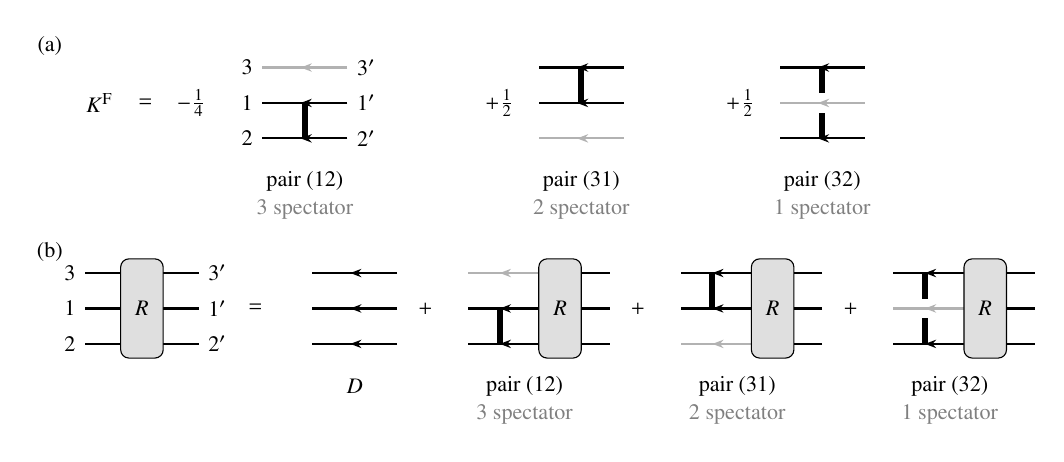
\begin{tikzpicture}[scale=0.9,every node/.style={font=\footnotesize},
  ln/.style={thick,postaction={decorate},decoration={markings,mark=at position 0.55 with {\arrow{Stealth[length=4pt]}}}},
  sp/.style={thick,gray!60,postaction={decorate},decoration={markings,mark=at position 0.55 with {\arrow{Stealth[length=4pt]}}}},
  br/.style={preaction={draw,white,line width=7pt}},
  vx/.style={line width=2.2pt},
  blob/.style={draw,fill=gray!25,rounded corners=3pt}]
% y positions: line 3 top, 1 middle, 2 bottom
\def\yt{1.0}\def\ym{0.5}\def\yb{0.0}
%------------- row (a): Faddeev kernel, Eq. (Faddeev)
\begin{scope}[yshift=2.9cm]
\node at (-0.9,1.3) {(a)};
\node at (-0.2,0.5) {$K^{\rm F}$}; \node at (0.45,0.5) {$=$};
\node at (1.10,0.5) {$-\tfrac14$};
\draw[sp] (3.30,\yt) -- (2.10,\yt);
\draw[ln] (3.30,\ym) -- (2.10,\ym);
\draw[ln] (3.30,\yb) -- (2.10,\yb);
\draw[vx] (2.70,\ym) -- (2.70,\yb);
\node[left] at (2.10,\yt) {3}; \node[left] at (2.10,\ym) {1}; \node[left] at (2.10,\yb) {2};
\node[right] at (3.30,\yt) {$3'$}; \node[right] at (3.30,\ym) {$1'$}; \node[right] at (3.30,\yb) {$2'$};
\node at (2.70,-0.6) {pair (12)};
\node[gray] at (2.70,-1.0) {3 spectator};
\node at (5.45,0.5) {$+\tfrac12$};
\draw[ln] (7.20,\yt) -- (6.00,\yt);
\draw[ln] (7.20,\ym) -- (6.00,\ym);
\draw[sp] (7.20,\yb) -- (6.00,\yb);
\draw[vx] (6.60,\yt) -- (6.60,\ym);
\node at (6.60,-0.6) {pair (31)};
\node[gray] at (6.60,-1.0) {2 spectator};
\node at (8.85,0.5) {$+\tfrac12$};
\draw[ln] (10.60,\yt) -- (9.40,\yt);
\draw[ln] (10.60,\yb) -- (9.40,\yb);
\draw[vx] (10.00,\yt) -- (10.00,\yb);
\draw[sp,br] (10.60,\ym) -- (9.40,\ym);
\node at (10.00,-0.6) {pair (32)};
\node[gray] at (10.00,-1.0) {1 spectator};
\end{scope}
%------------- row (b): Dyson equation
\node at (-0.9,1.3) {(b)};

%------------- R
\begin{scope}[xshift=0cm]
\draw[ln] (1.2,\yt) -- (-0.4,\yt); \draw[ln] (1.2,\ym) -- (-0.4,\ym); \draw[ln] (1.2,\yb) -- (-0.4,\yb);
\draw[blob] (0.1,-0.2) rectangle (0.7,1.2); \node at (0.4,0.5) {$R$};
\node[left] at (-0.4,\yt) {3}; \node[left] at (-0.4,\ym) {1}; \node[left] at (-0.4,\yb) {2};
\node[right] at (1.2,\yt) {$3'$}; \node[right] at (1.2,\ym) {$1'$}; \node[right] at (1.2,\yb) {$2'$};
\end{scope}
\node at (2.0,0.5) {$=$};
%------------- D
\begin{scope}[xshift=2.8cm]
\draw[ln] (1.2,\yt) -- (0,\yt); \draw[ln] (1.2,\ym) -- (0,\ym); \draw[ln] (1.2,\yb) -- (0,\yb);
\node at (0.6,-0.6) {$D$};
\end{scope}
\node at (4.4,0.5) {$+$};
%------------- V_alpha R
\begin{scope}[xshift=5.0cm]
\draw[sp] (1.0,\yt) -- (0,\yt);
\draw[thick] (2.0,\yt) -- (1.6,\yt);
\draw[ln] (1.0,\ym) -- (0,\ym);
\draw[thick] (2.0,\ym) -- (1.6,\ym);
\draw[ln] (1.0,\yb) -- (0,\yb);
\draw[thick] (2.0,\yb) -- (1.6,\yb);
\draw[vx] (0.45,\ym) -- (0.45,\yb);
\draw[blob] (1.0,-0.2) rectangle (1.6,1.2); \node at (1.3,0.5) {$R$};
\node at (0.8,-0.6) {pair (12)};
\node[gray] at (0.8,-1.0) {3 spectator};
\end{scope}
\node at (7.4,0.5) {$+$};
\begin{scope}[xshift=8.0cm]
\draw[ln] (1.0,\yt) -- (0,\yt);
\draw[thick] (2.0,\yt) -- (1.6,\yt);
\draw[ln] (1.0,\ym) -- (0,\ym);
\draw[thick] (2.0,\ym) -- (1.6,\ym);
\draw[sp] (1.0,\yb) -- (0,\yb);
\draw[thick] (2.0,\yb) -- (1.6,\yb);
\draw[vx] (0.45,\yt) -- (0.45,\ym);
\draw[blob] (1.0,-0.2) rectangle (1.6,1.2); \node at (1.3,0.5) {$R$};
\node at (0.8,-0.6) {pair (31)};
\node[gray] at (0.8,-1.0) {2 spectator};
\end{scope}
\node at (10.4,0.5) {$+$};
\begin{scope}[xshift=11.0cm]
\draw[ln] (1.0,\yt) -- (0,\yt);
\draw[thick] (2.0,\yt) -- (1.6,\yt);
\draw[thick] (2.0,\ym) -- (1.6,\ym);
\draw[ln] (1.0,\yb) -- (0,\yb);
\draw[thick] (2.0,\yb) -- (1.6,\yb);
\draw[vx] (0.45,\yt) -- (0.45,\yb);
\draw[sp,br] (1.0,\ym) -- (0,\ym);
\draw[blob] (1.0,-0.2) rectangle (1.6,1.2); \node at (1.3,0.5) {$R$};
\node at (0.8,-0.6) {pair (32)};
\node[gray] at (0.8,-1.0) {1 spectator};
\end{scope}
\end{tikzpicture}
\caption{(a) The Faddeev kernel, Eq.~\eqref{eq:Faddeev}. Lines run
from the second triple on the right to the first triple on the left.
The thick bar is the two-particle vertex $\Gamma^{\pp}$: it connects the
two lines of one pair, while the third line (gray) is a spectator. Its
factor $G^{-1}$ cancels one line of $D$ or $R$ when the kernel is
inserted into Eq.~\eqref{eq:R}, so that the spectator passes the vertex
without interacting. (b) The Dyson equation for $R$, Eq.~\eqref{eq:R},
with the Faddeev kernel of panel (a), sorted by the interacting pair.
The exchange of the lines 1 and 2 in $D$ is implied.}
\label{fig:Faddeev_pairs}
\end{figure*}

Substituting Eq.~\eqref{eq:Faddeev} directly into the Dyson equation, Eq.~\eqref{eq:R},
and closing the spectator leg of each of the three terms against the
corresponding $G^{-1}$ gives
\begin{align}
R(312;1'2'3')
={}&
D(312;1'2'3')
\nonumber\\
&-
\frac14\,
\big[
G(1\bar1)\,G(2\bar2)
-
G(1\bar2)\,G(2\bar1)
\big]
\nonumber\\
&\quad\times
\Gamma^{\pp}(\bar1\bar2;\bar1'\bar2')\,
R(3\bar1'\bar2';1'2'3')
\nonumber\\
&+
\frac12\,
G(3\bar3)\,
\Big[
G(1\bar1)\,\Gamma^{\pp}(\bar3\bar1;\bar1'\bar3')
\nonumber\\
&\hphantom{+\tfrac12\,G(3\bar3)\,\Big[}
\times
R(\bar3'\bar1'2;1'2'3')
\nonumber\\
&\hphantom{+\tfrac12\,G(3\bar3)\,\Big[}
-
G(2\bar1)\,\Gamma^{\pp}(\bar3\bar1;\bar1'\bar3')
\nonumber\\
&\hphantom{+\tfrac12\,G(3\bar3)\,\Big[}
\times
R(\bar3'\bar1'1;1'2'3')
\Big]
\nonumber\\
&+
\frac12\,
G(3\bar3)\,
\Big[
G(2\bar2)\,\Gamma^{\pp}(\bar3\bar2;\bar2'\bar3')
\nonumber\\
&\hphantom{+\tfrac12\,G(3\bar3)\,\Big[}
\times
R(\bar3'1\bar2';1'2'3')
\nonumber\\
&\hphantom{+\tfrac12\,G(3\bar3)\,\Big[}
-
G(1\bar2)\,\Gamma^{\pp}(\bar3\bar2;\bar2'\bar3')
\nonumber\\
&\hphantom{+\tfrac12\,G(3\bar3)\,\Big[}
\times
R(\bar3'2\bar2';1'2'3')
\Big].
\label{eq:R_parquet}
\end{align}
In $\Sigma^{c}$, Eq.~\eqref{eq:Sigma_3}, labelled along its time-ordered chains (Sec.~\ref{sec:time_orderings}), line 3 becomes the hole for
$t_{1'}<t_1$ (block II) or the particle for $t_1<t_{1'}$ (block I). The
pairs $(31)$ and $(32)$ then give the ring-type self-energy diagrams,
labelled $\eh$ and $\teh$ below.
Inserting Eq.~\eqref{eq:R_parquet} into
Eq.~\eqref{eq:Sigma_3} gives the channel decomposition of the
self-energy
\begin{equation}
\Sigma^{c}(11')
=
\Sigma^{(2)}(11')
+
\Sigma^{c}_{\pp}(11')
+
\Sigma^{c}_{\eh}(11')
+
\Sigma^{c}_{\teh}(11'),
\label{eq:Sigma_parquet}
\end{equation}
where $\Sigma^{c}_{\pp}$, $\Sigma^{c}_{\eh}$ and $\Sigma^{c}_{\teh}$
collect the terms of Eq.~\eqref{eq:R_parquet} in which the last
interaction acts on the pair $(12)$, $(31)$ and $(32)$, respectively.
The first term on the
\emph{r.h.s.} is recognized to be the 
GF2 self-energy,
\begin{equation}
	\label{eq:Sigma_D}
\begin{aligned}
\Sigma^{(2)}(11')
={}&
v(1\bar2;\bar3'\bar2')\,
G(\bar3'\bar4)\,
\big[
v(\bar4\bar5;1'\bar6')
-
v(\bar4\bar5;\bar6'1')
\big]
\\
&\times
G(\bar6'\bar2)\,
G(\bar2'\bar5^+) \;.
\end{aligned}
\end{equation}
We now eliminate $R$.
We write Eq.~\eqref{eq:R_parquet} as an operator
equation on $R$'s first triple,
\begin{equation}
R = D + \cK R,
\qquad
\cK \equiv D\,K^{\rm F} \;,
\label{eq:K_def}
\end{equation}
where the spectator line of each term of $K^{\rm F}$ is closed against
its $G^{-1}$, as in Eq.~\eqref{eq:R_parquet}.
The identity in the $\pph$ space, \ie\ the
$G\to\delta$ limit of $D$, is
\begin{equation}
\delta_{\pph}(312;1'2'3')
=
\delta(3,3')
\big[
\delta(1,1')\,\delta(2,2')
-
\delta(1,2')\,\delta(2,1')
\big] \;.
\label{eq:delta_pph}
\end{equation}
Solving Eq.~\eqref{eq:K_def} for $R$,
\begin{equation}
	\label{eq:R_inverse}
R(312;1'2'3')
=
\big[(\bI-\cK)^{-1}D\big](312;1'2'3'),
\end{equation}
which is shorthand for the
Neumann series
\begin{align}
(\bI-\cK)^{-1}(312;1'2'3')
={}&
\delta_{\pph}(312;1'2'3')
+
\cK(312;1'2'3')
\nonumber\\
&+
\cK(312;\bar3\bar1\bar2)\,
\cK(\bar3\bar1\bar2;1'2'3')
\nonumber\\
&+
\cdots.
\label{eq:K_series}
\end{align}
Eq.~\eqref{eq:R_inverse} eliminates $R$ 
by expressing it in terms of $D$ (i.e. $G$) and $\cK$
(i.e. $\Gamma^{\pp}$). Substituting
Eq.~\eqref{eq:R_inverse} into Eq.~\eqref{eq:Sigma_3} 
\begin{align}
\Sigma^{c}(11')
={}&
v(1\bar2;\bar3'\bar2')\,
G(\bar3'\bar4)\,
v(\bar4\bar5;\bar6'\bar7')
\nonumber\\
&\times
\big[(\bI-\cK)^{-1}D\big](\bar2'\bar6'\bar7';\bar3\bar2\bar5^+)\,
G^{-1}(\bar3 1') \;.
\label{eq:Sigma_closed}
\end{align}
At zeroth order in $\cK$, Eq.~\eqref{eq:Sigma_D} is 
recovered, and beyond zeroth order in $\cK$ it resums
$\Sigma^{c}_{\pp}+\Sigma^{c}_{\eh}
+\Sigma^{c}_{\teh}$ to all orders, with $R$ eliminated
throughout. Eq.~\eqref{eq:Sigma_closed}
is the three-particle analogue of the Schwinger--Dyson
equation, Eq.~\eqref{eq:SDE_G2}.

\subsection{Expansion of the Faddeev kernel}
The next useful step is to expand the Faddeev kernel order by order in 
$\bar{v}$.  
\label{sec:K_expansion}
\begin{equation}
\cK
=
\cK^{(1)}+\cK^{(2)}+\cK^{(3)}+O(v^4).
\label{eq:K_expansion}
\end{equation}
\subsubsection{Vertices}
At first order, all channels contain only the bare antisymmetrized
interaction,
\begin{align}
\Gamma^{\pp,(1)}
&=
\Gamma^{\eh,(1)}
=
\Gamma^{\teh,(1)}
=
\Lambda^{(1)}
\equiv
\Gamma^{(1)},
\nonumber\\
\Gamma^{(1)}(12;1'2')
&=
-\ii\,\bar v(12;1'2'),
\nonumber\\
\bar v(12;1'2')
&\equiv
v(12;1'2')-v(12;2'1') \;.
\label{eq:Gamma1_bare}
\end{align}
To all orders,
\begin{align}
\Gamma^{\eh}
&=
\Lambda+\Phi^{\teh}+\Phi^{\pp},
\nonumber\\
\Gamma^{\teh}
&=
\Lambda+\Phi^{\eh}+\Phi^{\pp},
\nonumber\\
\Gamma^{\pp}
&=
\Lambda+\Phi^{\eh}+\Phi^{\teh},
\nonumber\\
F
&=
\Gamma^{r}+\Phi^{r}
=
\Lambda+\Phi^{\pp}+\Phi^{\eh}+\Phi^{\teh} \;.
\label{eq:parquet_channels}
\end{align}
Note that\cite{MarieLoos2025}
\begin{equation}
\Lambda = \Lambda^{(1)}+O(v^4) \;.
\label{eq:crossing_Lambda}
\end{equation}
Defining 
\begin{align}
(A\circ_{\pp} B)(12;1'2')
&\equiv
A(12;\bar1\bar2)\,G(\bar1\bar1')\,G(\bar2\bar2')
\nonumber\\
&\hphantom{\equiv}\times
B(\bar1'\bar2';1'2'),
\label{eq:circ_def}
\\
(A\circ_{\eh}B)(12;1'2')
&\equiv
A(1\bar4;1'\bar3)\,G(\bar3\bar3')\,G(\bar4'\bar4)
\nonumber\\
&\hphantom{\equiv}\times
B(\bar3'2;\bar4'2'),
\label{eq:circ_eh_def}
\end{align}
the $\pp$ and $\eh$ BSEs are\cite{Kugler2018} 
\begin{equation}
	\begin{aligned}
F
={}&
\Gamma^{\pp}-\frac12\,\Gamma^{\pp}\circ_{\pp} F \;, \\
F
={}&
\Gamma^{\eh}+\Gamma^{\eh}\circ_{\eh}F \;.
\label{eq:parquet_BSE}
	\end{aligned}
\end{equation}
At second order, the reducible vertices are
\begin{equation}
	\begin{aligned}
\Phi^{\eh,(2)}
={}&
\Gamma^{(1)}\circ_{\eh}\Gamma^{(1)}, \\
\Phi^{\pp,(2)}
={}&
-\frac12\,\Gamma^{(1)}\circ_{\pp}\Gamma^{(1)},
\label{eq:Phi2_explicit}
	\end{aligned}
\end{equation}
and at third order 
\begin{equation}
	\begin{aligned}
\Phi^{\eh,(3)}
={}&
\Gamma^{\eh,(2)}\circ_{\eh}\Gamma^{(1)}
+\Gamma^{(1)}\circ_{\eh}\Gamma^{\eh,(2)}
\\
&+\Gamma^{(1)}\circ_{\eh}\Gamma^{(1)}\circ_{\eh}\Gamma^{(1)},
\\
\Phi^{\pp,(3)}
={}&
-\frac12\big(\Gamma^{\pp,(2)}\circ_{\pp}\Gamma^{(1)}
+\Gamma^{(1)}\circ_{\pp}\Gamma^{\pp,(2)}\big)
\\
&+\frac14\,\Gamma^{(1)}\circ_{\pp}\Gamma^{(1)}\circ_{\pp}\Gamma^{(1)}.
\label{eq:Phi3_st}
\end{aligned} 
\end{equation}
Together with Eqs.~\eqref{eq:parquet_channels} and
\eqref{eq:crossing_Lambda} and fermionic crossing,
\begin{equation}
\Phi^{\teh}(12;1'2')
=
-\Phi^{\eh}(21;1'2') \;,
\label{eq:crossing}
\end{equation}
this gives $\Gamma^{r,(2)}$ and $\Gamma^{r,(3)}$.

\subsubsection{Pair operators}
Let us now investigate Eq.~\eqref{eq:R_parquet} 
in more detail. There, the terms are sorted by the three terms of
Eq.~\eqref{eq:Faddeev}. It is, however, useful to sort them by the pairs
$\alpha=(12),(31),(32)$ of incoming lines that interact. For any
4-point $Y$ and any $\chi$ antisymmetric in its first pair,
\begin{align}
\big[\cK_{12}[Y]\chi\big](312;1'2'3')
={}&
-\frac14\big[G(1\bar1)G(2\bar2)-G(1\bar2)G(2\bar1)\big]
\nonumber\\
&\times
Y(\bar1\bar2;\bar1'\bar2')\,\chi(3\bar1'\bar2';1'2'3'),
\nonumber\\
\big[\cK_{31}[Y]\chi\big](312;1'2'3')
={}&
G(3\bar3)\,G(1\bar1)\,Y(\bar3\bar1;\bar1'\bar3')
\nonumber\\
&\times
\chi(\bar3'\bar1'2;1'2'3'),
\nonumber\\
\big[\cK_{32}[Y]\chi\big](312;1'2'3')
={}&
G(3\bar3)\,G(2\bar2)\,Y(\bar3\bar2;\bar2'\bar3')
\nonumber\\
&\times
\chi(\bar3'1\bar2';1'2'3').
\label{eq:pair_ops}
\end{align}
The first term of Eq.~\eqref{eq:R_parquet} is $\cK_{12}[\Gamma^{\pp}]$.
The second term of each bracket in Eq.~\eqref{eq:R_parquet} acts on
the other pair, since $R$ is antisymmetric in 1 and 2. Each of the
pairs $(31)$ and $(32)$ therefore receives $\tfrac12$ from each
bracket, and the Faddeev kernel becomes
\begin{equation}
\cK
=
\cK_{12}\big[\Gamma^{\pp}\big]
+\cK_{31}\big[\Gamma^{\pp}\big]
+\cK_{32}\big[\Gamma^{\pp}\big] \;.
\label{eq:K_pairs}
\end{equation}
Cutting the two lines of pair $\alpha$ separates the outgoing from the
incoming legs of $Y$ in $\cK_\alpha[Y]$, \ie\ all three pairs scatter
in the $\pp$ channel of $R$.

Eq.~\eqref{eq:K_pairs} is the kernel of Barbieri and
Dickhoff.\cite{Barbieri2001} It is exact at first order, where all
vertices are $\Gamma^{(1)}$. Beyond first order, iterating $\cK_{3x}[\Gamma^{\pp}]$ alone would
count the rungs of the ladders in the pairs $(31)$ and $(32)$ twice,
since $D$ is not antisymmetrized in the lines 3 and $x$. The $\pp$ channel of $R$ in the pair $(3x)$ is the $\eh$ channel of $F$, whose ladder $\Phi^{\eh}$ is already contained in $\Gamma^{\pp}$. We therefore
replace $\Gamma^{\pp}$ in $\cK_\alpha$ by a pair vertex $\Gamma_\alpha$,
fixed such that the pair $\alpha$ alone reproduces its full two-body
scattering $F$. For the pair $(12)$, $\Gamma_{12}=\Gamma^{\pp}$, and at
first order $\Gamma_\alpha=\Gamma^{(1)}$ for all pairs. Their explicit form is not needed,
since only $F$ appears in the Faddeev form derived next.

\subsection{\label{sec:Faddeev_form}Faddeev form of Eq.~\eqref{eq:Sigma_closed}: the ADC--parquet link}
In Sec.~\ref{sec:K_expansion}, we have written the Faddeev kernel in
terms of two-particle irreducible vertices in the pairs. This form is convenient for expanding
Eq.~\eqref{eq:Sigma_closed} order by order.
The aim of this subsection is to rewrite Eq.~\eqref{eq:Sigma_closed} such
that only the full vertex $F$ appears in all three pairs.
This is the Faddeev form of the three-body problem.\cite{Faddeev1961}

Based on the Faddeev construction, we will then show that 
GF$n$ is the truncation of the Faddeev series,
at total order $n-2$ in $v$. 
The ADC($n$) matrices then
follow from Schirmer's matching,\cite{Schirmer1983} in which the
resolvent form of ADC($n$) is imposed and matched to the self-energy
order by order. ADC(3) is worked out as an
illustrative case in App.~\ref{app:ADC}.

Parquet at fixed order is merely a laborious way to
derive ADC. The link becomes nontrivial once $F$ is kept resummed,
in which case 
the Faddeev series defines approximations beyond any
fixed order in terms of the parquet vertex.
It is the purpose of Sec.~\ref{sec:parquet_Heff} to bring the resulting 
self-energies into effective-Hamiltonian form.


\subsubsection{Splitting $R$ by the last interacting pair}
With the kernel sorted by pairs, Eq.~\eqref{eq:K_pairs}, and the pair
vertices $\Gamma_\alpha$, the Dyson equation for $R$,
Eq.~\eqref{eq:K_def}, reads
\begin{equation}
R=D+\sum_{\alpha}\mathcal V_\alpha R \;,
\qquad
\mathcal V_\alpha=\cK_\alpha\big[\Gamma_\alpha\big] \;,
\label{eq:Dyson_pairs}
\end{equation}
where $\mathcal V_\alpha$ acts only on the pair $\alpha$, with the
third line as a free spectator [Fig.~\ref{fig:Faddeev_pairs}(b), with
the thick bars standing for $\Gamma_\alpha$]. In block II,
$\mathcal V_{12}$ is particle--particle scattering with the hole as
spectator, and $\mathcal V_{31}$, $\mathcal V_{32}$ are particle--hole
scattering with one of the particles as spectator.
We collect the terms of $R$ in which the last interaction, \ie\ the
one closest to the outgoing triple, acts on the pair $\alpha$ into
$R_\alpha\equiv\mathcal V_\alpha R$. Solving
$R_\alpha=\mathcal V_\alpha\big(D+R_\alpha+\sum_{\beta\neq\alpha}R_\beta\big)$
for $R_\alpha$ gives
\begin{equation}
\label{eq:Faddeev_rearr}
\begin{aligned}
R
= &
D+R_{12}+R_{31}+R_{32} \;,
\\
R_\alpha
= &
\big(\bI-\mathcal V_\alpha\big)^{-1}\mathcal V_\alpha
\Big(D+\sum_{\beta\neq\alpha}R_\beta\Big) \;,
\end{aligned}
\end{equation}
where $(\bI-\mathcal V_\alpha)^{-1}\mathcal V_\alpha$ sums all
consecutive interactions in the pair $\alpha$.

Acting on $D$, $(\bI-\mathcal V_\alpha)^{-1}\mathcal V_\alpha$ gives all
diagrams of $R$ in which only the pair $\alpha$ interacts, while the
third line is a free spectator. By the definition of $\Gamma_\alpha$,
this is the full two-body scattering of the pair,
$\cK_\alpha[F]=\mathcal V_\alpha+\mathcal V_\alpha\cK_\alpha[F]$,
so that
\begin{equation}
\big(\bI-\mathcal V_\alpha\big)^{-1}\mathcal V_\alpha
=
\cK_\alpha[F] \;.
\label{eq:V_to_F}
\end{equation}
Inserting
Eq.~\eqref{eq:V_to_F} into
Eq.~\eqref{eq:Faddeev_rearr} gives the Faddeev
equations\cite{Barbieri2001}
\begin{equation}
\label{eq:Faddeev_F}
R_\alpha
=
\cK_\alpha[F]\Big(D+\sum_{\beta\neq\alpha}R_\beta\Big) \;.
\end{equation}
Iterating Eq.~\eqref{eq:Faddeev_F}, \ie\ inserting the $R_\beta$ on
the right-hand side again and again, gives the Faddeev series
\cite{watson1953multiple,Faddeev1961,Barbieri2001}
\begin{equation}
\label{eq:Faddeev_series}
\begin{aligned}
R
= &
D+\sum_{\alpha}\cK_\alpha[F]D
+\sum_{\alpha\neq\beta}\cK_\alpha[F]\cK_\beta[F]D
\\
& +\sum_{\substack{\alpha\neq\beta\\\beta\neq\gamma}}
\cK_\alpha[F]\cK_\beta[F]\cK_\gamma[F]D+\cdots \;,
\end{aligned}
\end{equation}
in which consecutive pairs are always different.

To relate Eq.~\eqref{eq:Faddeev_series} to ADC, we expand $F$ in powers
of $v$. By Eqs.~\eqref{eq:parquet_channels} and
\eqref{eq:crossing_Lambda}, $\Lambda$ has no second-order term,
so that
\begin{equation}
\label{eq:F_orders}
\begin{aligned}
F^{(1)}
= &
\Gamma^{(1)} \;,
\\
F^{(2)}
= &
\Phi^{\pp,(2)}+\Phi^{\eh,(2)}+\Phi^{\teh,(2)} \;.
\end{aligned}
\end{equation}
The self-energy, Eq.~\eqref{eq:Sigma_closed}, contains two explicit
interactions $v$. A term of order $m$ in $v$ therefore contributes to
$\Sigma$ at order $m+2$. ADC($n$) is complete through order $n$, so
that $R$ is needed through order $n-2$ in $v$. Collecting the terms of
Eq.~\eqref{eq:Faddeev_series} up to this order,
\begin{equation}
\label{eq:ADC_Faddeev}
\begin{aligned}
R_{\rm ADC(2)}
= &
D \;,
\\
R_{\rm ADC(3)}
= &
D+\sum_{\alpha}\cK_\alpha\big[F^{(1)}\big]D_{\rm HF} \;,
\\
R_{\rm ADC(4)}
= &
D+\sum_{\alpha}\cK_\alpha\big[F^{(1)}+F^{(2)}\big]D_{\rm HF}
\\
& +\sum_{\alpha\neq\beta}
\cK_\alpha\big[F^{(1)}\big]\cK_\beta\big[F^{(1)}\big]D_{\rm HF} \;.
\end{aligned}
\end{equation}
Here, $D$ in the first term, $G(\bar3'\bar4)$ and the static part
$\Sigma_{\rm HF}$ are evaluated with $G$ expanded to the corresponding
order, while in all terms with at least one $F$, $D_{\rm HF}$ suffices
at this order.

Before concluding this section,
we introduce the important own-channel approximation
to Eq.~\eqref{eq:Faddeev_series}.
For this, we approximate the BSEs Eq.~\eqref{eq:parquet_BSE}
in the own-channel approximation, for the special case of 
the first-order Faddeev kernel, so that 
$\Gamma^{r}\to\Gamma^{(1)}$.
The two BSEs then define two separate vertices
\begin{equation}
\begin{aligned}
F^{\pp}_{\rm oc}
= &
\Gamma^{(1)}-\frac12\,\Gamma^{(1)}\circ_{\pp}F^{\pp}_{\rm oc} \;,
\\
F^{\eh}_{\rm oc}
= &
\Gamma^{(1)}+\Gamma^{(1)}\circ_{\eh}F^{\eh}_{\rm oc} \;.
\end{aligned}
\label{eq:BSE_oc}
\end{equation}
This is also done in the FLEX approximation.\cite{Bickers1989,Bickers2004}

In the own-channel approximation to Eq.~\eqref{eq:Faddeev_series},
each pair scatters only through the
ladder of its own channel with the bare kernel. 
The own-channel approximation amounts to 
neglecting the channel crossings of
parquet (and of coupled cluster) inside a pair.\cite{Barbieri2001}
\citet{Barbieri2001} combined this approximation additionally with
a no-overlap approximation that we denote here by 
$[\cdots]_{\pph}$. It neglects the time orderings in which the ladders of
different pairs overlap in time, \ie\ consecutive pairs are separated by
a $\pph$ cut, a subinterval spanned only by the three lines of a $\pph$
state (Sec.~\ref{sec:pph_Dyson}). 
Due to this restriction, at first-order Faddeev the effective
Hamiltonian only contains $\pph$ ($\hhp$) configurations.
At fourth order, the neglected terms are
added perturbatively together with the $3\text{p}2\text{h}$
($3\text{h}2\text{p}$) space.
With these approximations, Eq.~\eqref{eq:Faddeev_series} becomes 
\begin{equation}
\label{eq:Faddeev_series_oc}
\begin{aligned}
R_{\rm oc}
= &
D+\sum_{\alpha}\cK_\alpha[F_\alpha]D
+\sum_{\alpha\neq\beta}\Big[\cK_\alpha[F_\alpha]\cK_\beta[F_\beta]D\Big]_{\pph}
\\
& +\sum_{\substack{\alpha\neq\beta\\\beta\neq\gamma}}
\Big[\cK_\alpha[F_\alpha]\cK_\beta[F_\beta]\cK_\gamma[F_\gamma]D\Big]_{\pph}
+\cdots \;.
\end{aligned}
\end{equation}

\begin{figure*}
\centering
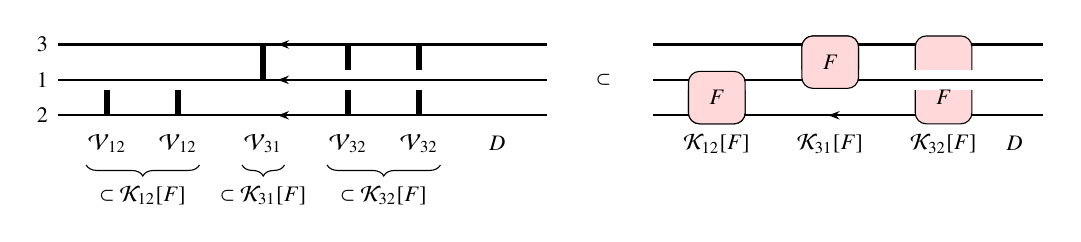
\begin{tikzpicture}[scale=0.9,every node/.style={font=\footnotesize},
  ln/.style={thick,postaction={decorate},decoration={markings,mark=at position 0.55 with {\arrow{Stealth[length=4pt]}}}},
  pl/.style={thick},
  br/.style={preaction={draw,white,line width=7pt}},
  vx/.style={line width=2.2pt},
  Fb/.style={draw,fill=red!15,rounded corners=4pt}]
\def\yt{1.0}\def\ym{0.5}\def\yb{0.0}
%------------- row: V12 V12 V31 V32 V32 D
\begin{scope}
\draw[ln] (6.6,\yt) -- (-0.3,\yt); \draw[ln] (6.6,\yb) -- (-0.3,\yb);
% vertices at x = 0.4 (12), 1.4 (12), 2.6 (31), 3.8 (32), 4.8 (32)
\draw[vx] (0.4,\yb) -- (0.4,\ym);
\draw[vx] (1.4,\yb) -- (1.4,\ym);
\draw[vx] (2.6,\ym) -- (2.6,\yt);
\draw[vx] (3.8,\yb) -- (3.8,\yt);
\draw[vx] (4.8,\yb) -- (4.8,\yt);
\draw[ln,br] (6.6,\ym) -- (-0.3,\ym);
\draw[vx] (2.6,\ym) -- (2.6,\yt);
\node[left] at (-0.3,\yt) {3}; \node[left] at (-0.3,\ym) {1}; \node[left] at (-0.3,\yb) {2};
\node at (0.4,-0.4) {$\mathcal V_{12}$}; \node at (1.4,-0.4) {$\mathcal V_{12}$};
\node at (2.6,-0.4) {$\mathcal V_{31}$}; \node at (3.8,-0.4) {$\mathcal V_{32}$};
\node at (4.8,-0.4) {$\mathcal V_{32}$}; \node at (5.9,-0.4) {$D$};
\draw[decorate,decoration={brace,mirror,amplitude=4pt}] (0.1,-0.7) -- (1.7,-0.7) node[midway,below=4pt] {$\subset\cK_{12}[F]$};
\draw[decorate,decoration={brace,mirror,amplitude=4pt}] (2.3,-0.7) -- (2.9,-0.7) node[midway,below=4pt] {$\subset\cK_{31}[F]$};
\draw[decorate,decoration={brace,mirror,amplitude=4pt}] (3.5,-0.7) -- (5.1,-0.7) node[midway,below=4pt] {$\subset\cK_{32}[F]$};
\end{scope}
\node at (7.4,0.5) {$\subset$};
%------------- row: K12[F] K31[F] K32[F] D
\begin{scope}[xshift=8.4cm]
\draw[ln] (5.2,\yt) -- (-0.3,\yt); \draw[ln] (5.2,\yb) -- (-0.3,\yb);
\draw[Fb] (0.2,-0.12) rectangle (1.0,0.62); \node at (0.6,0.25) {$F$};
\draw[Fb] (1.8,0.38) rectangle (2.6,1.12); \node at (2.2,0.75) {$F$};
\draw[Fb] (3.4,-0.12) rectangle (4.2,1.12);
\draw[ln,br] (5.2,\ym) -- (-0.3,\ym);
\draw[Fb] (1.8,0.38) rectangle (2.6,1.12); \node at (2.2,0.75) {$F$};
\draw[Fb] (0.2,-0.12) rectangle (1.0,0.62); \node at (0.6,0.25) {$F$};
\node at (3.8,0.25) {$F$};
\node at (0.6,-0.4) {$\cK_{12}[F]$}; \node at (2.2,-0.4) {$\cK_{31}[F]$};
\node at (3.8,-0.4) {$\cK_{32}[F]$}; \node at (4.8,-0.4) {$D$};
\end{scope}
\end{tikzpicture}
\caption{Regrouping of the Neumann series, Eq.~\eqref{eq:K_series}, into
the Faddeev series. Left: one term of the Neumann series, a sequence of
pair vertices $\mathcal V_\alpha$ (thick bars). Right: each run of
consecutive vertices in the same pair is part of the full two-body
scattering $\cK_\alpha[F]$ of that pair (shaded box), so that
consecutive boxes always belong to different pairs.}
\label{fig:Faddeev_runs}
\end{figure*}

\section{\label{sec:parquet_Heff}Parquet in effective-Hamiltonian form}
In this section, by making use of the own-channel
and no-overlap approximation
we have just introduced, we replace the 
Tamm--Dancoff ladders of each pair in the $\pph$ propagator
by full RPA ladders. At the level of
ADC(3), this is essentially the Faddeev random-phase approximation
(FRPA) of Barbieri and co-workers.
\cite{Barbieri2001,
barbieri2003extension,
barbieri2007quasiparticles,
Degroote2011}
The difference is that our effective Hamiltonian remains Hermitian,
as long as its metric is positive definite.
At the level of ADC(4), it is, to our knowledge, new.

To make this section self-contained, we need to introduce 
the time-ordering rules for instantaneous interactions,
the pair propagators, and the
$\pph$ Dyson equation. With these tools, we can 
construct the reducible vertices of order $n$ in their 
own-channel approximations. We then derive the effective 
Hamiltonians of the 3rd- and 4th-order own-channel and no-overlap parquet approximations, 
i.e. Faddeev-RPA and its completion to fourth order.

Let us stress that, the own-channel and no-overlap approximations aside, 
a couple of other approximations are made by construction.
The first one is the parquet approximation, that replaces 
the fully irreducible vertex by the bare interaction, $\Lambda=\Gamma^{(1)}$.
Since $\Lambda=\Lambda^{(1)}+O(v^4)$, Eq.~\eqref{eq:crossing_Lambda}, $F$ is
exact through third order. 
We also employ a static HF reference throughout, i.e. all lines of the vertex are
$G_{\rm HF}$. The lines of $D$ are dressed through the self-energy
order by order, in the same way as in ADC. With these approximations, every diagram of the vertex is a
product of instantaneous interactions $\bar v$ and $G_{\rm HF}$ lines.
The time-ordering rules then remove all three frequencies of the vertex.
This makes an effective-Hamiltonian form possible.
Whether it is possible to obtain an effective Hamiltonian form 
also beyond the parquet approximation is an open question.

Finally, we make the Faddeev approximation, that consists in neglecting
the 3-body irreducible kernel. This
affects the self-energy from fifth order on.
Taken together, these approximations restrict the construction of 
order-complete self-energies through $n=4$. 


\subsection{Notation and time-orderings}
\label{sec:time_orderings}
We use real canonical spin-orbitals and map numbers to orbitals
with $1,2,1',2'\to p,q,r,s$.
Since $\bar v$ is instantaneous,
\begin{equation}
\bar v(12;1'2')
\to
\mel{pq}{}{rs}\,
\delta(t_1-t_2)\,\delta(t_1-t_{1'})\,\delta(t_2-t_{2'}),
\label{eq:vbar_orbital}
\end{equation}
with
\begin{equation}
\mel{pq}{}{rs} =
\braket{pq}{rs}-\braket{pq}{sr} \;.
\label{eq:mel_def}
\end{equation}
We will use a HF reference, 
\begin{equation}
G_{\rm HF}^{-1}=G_0^{-1}-\Sigma_{\rm HF}[G_{\rm HF}] \;.
\label{eq:G_HF}
\end{equation}
In canonical spin-orbitals $p$ with energies $\eps_p$, occupations
$n_p$ ($n_i=1$, $n_a=0$, $\bar n_p=1-n_p$), and $\sigma_p=+1$ for
virtual and $\sigma_p=-1$ for occupied orbitals,
\begin{equation}
G_{{\rm HF},p}(t)
=
-\ii\sigma_p\,\theta(\sigma_pt)\,e^{-\ii\eps_pt} \;.
\label{eq:G_sigma}
\end{equation}
Virtual lines run forward and occupied lines backward in time.
In frequencies,
\begin{equation}
	\label{eq:GHF_omega}
G_{{\rm HF},p}(\omega)
=
\frac{\bar n_p}{\omega-\eps_p+\ii0^+}
+
\frac{n_p}{\omega-\eps_p-\ii0^+}.
\end{equation}
We use the Fourier transform convention
\begin{equation}
\label{eq:fourier_transform}
G(\omega)
=
\int\dd t \;e^{\ii\omega t}\,G(t) \;,
\end{equation}
with $t = t_1 - t_{1'}$.
A useful identity is\cite{stefanucci2014diagrammatic} 
\begin{equation}
G_p(t_a-t_c)
=
\ii\sigma_p\,G_p(t_a-t_b)\,G_p(t_b-t_c),
\label{eq:line_cut}
\end{equation}
with $t_b$ between $t_a$ and $t_c$.

Since all interactions are instantaneous
(Eq.~\eqref{eq:vbar_orbital}), any integral over internal times
in any approximation to the Faddeev kernel can be evaluated
by Fourier transforming the product of its lines $\lambda$, with
orbitals $p_\lambda$. For $n$ internal times $\tau_1,\dots,\tau_n$ and the
external times $t_1$, $t_{1'}$, ordered as $T_0<T_1<\dots<T_{n+1}$,
\cite{fetter2012quantum}
\begin{align}
\prod_\lambda G_{p_\lambda}
={}&
\prod_\lambda\big(-\ii\sigma_{p_\lambda}\big)\,
e^{-\ii\sum_{k=1}^{n+1}E_k s_k},
\nonumber\\
E_k
={}&
\sum_{\lambda\,\text{spanning}\,(T_{k-1},T_k)}
\sigma_{p_\lambda}\,\eps_{p_\lambda} \;,
\label{eq:lemma_product_n}
\end{align}
with $s_k = T_k-T_{k-1}$. All $s_k$ are
independent integration variables,
and the Fourier transform Eq.~\eqref{eq:fourier_transform} factorizes,
\cite{fetter2012quantum}
\begin{align}
\mathcal F
={}&
\int\dd t\,e^{\ii\omega t}\!\int\dd\tau_1\cdots\dd\tau_n\,
e^{-\ii\sum_kE_ks_k}
=
\prod_{k=1}^{n+1}f_k,
\nonumber\\
f_k
={}&
\begin{cases}
\dfrac{\ii}{\omega-E_k}, & (T_{k-1},T_k)\subset(t_{1'},t_1),\\[1.2ex]
\dfrac{1}{\ii(\omega+E_k)}, & (T_{k-1},T_k)\subset(t_1,t_{1'}),\\[1.2ex]
\dfrac{1}{\ii E_k}, & \text{otherwise}.
\end{cases}
\label{eq:lemma_FT_n}
\end{align}
To attach the line factors of Eq.~\eqref{eq:lemma_product_n} to the
subintervals as well, a line spanning several subintervals is cut at
every vertex time it passes, Eq.~\eqref{eq:line_cut}. Every
subinterval then carries
$\prod(-\ii\sigma)$ of its own lines, and every vertex a factor
$\ii\sigma$ for each line that passes it without being attached.
We label an ordering by $(n_<,n_>;\ell_1,\dots)$: $n_<$ ($n_>$) internal
times before (after) the external interval, $\ell_k$ lines spanning
its $k$-th subinterval. These are the standard 
denominator rules for Goldstone diagrams.

\subsection{Pair propagators}
\label{sec:propagators}
All $G$ are the non-interacting $G_{\rm HF}$ as defined by Eqs.~\eqref{eq:G_sigma} and
\eqref{eq:GHF_omega} in this subsection.
\subsubsection{Non-interacting pair propagators}
The non-interacting pair propagators in the time domain are 
obtained from 
Eq.~\eqref{eq:G_sigma} and 
Eq.~\eqref{eq:lemma_product_n} as
\begin{equation}
L^{\pp}_{0,xy}(t)
= 
G_x(t)\,G_y(t)
=
-\delta_{\sigma_x\sigma_y}\,\theta(\sigma_xt)\,
e^{-\ii(\eps_x+\eps_y)t} \;,
\label{eq:L0pp_time}
\end{equation}
and 
\begin{equation}
L^{\eh}_{0,xr}(t)
= 
G_x(-t)\,G_r(t) =
\delta_{\sigma_x,-\sigma_r}\,\theta(\sigma_rt)\,
e^{-\ii(\eps_r-\eps_x)t} \;.
\label{eq:L0eh_time}
\end{equation}
In the frequency domain,
the particle-particle propagator is
\begin{equation}
\label{eq:L0pp_omega}
\begin{aligned}
L^{\pp}_{0,xy}(\Omega)
= &
\int\frac{\dd\nu}{2\pi}\,
G_x(\nu)\,G_y(\Omega-\nu)
\\
= &
\frac{-\ii\sigma_x\,\delta_{\sigma_x\sigma_y}}
{\Omega-(\eps_x+\eps_y)+\ii\sigma_x0^+} \;,
\end{aligned}
\end{equation}
with its indices restricted to 
$(xy)\in\big\{(cd),\,c<d\big\}\cup\big\{(kl),\,k<l\big\}$.
The particle-hole propagator is
\begin{equation}
\label{eq:L0eh_omega}
\begin{aligned}
L^{\eh}_{0,xr}(\Omega)
= & 
\int\frac{\dd\nu}{2\pi}\,
G_x(\nu)\,G_r(\nu+\Omega)
\\
= &
\frac{\ii\sigma_r\,\delta_{\sigma_x,-\sigma_r}}
{\Omega-(\eps_r-\eps_x)+\ii\sigma_r0^+} \;,
\end{aligned}
\end{equation}
with its indices restricted to 
$(xr)\in\big\{(ia)\big\}\cup\big\{(ai)\big\}$.

\subsubsection{Interacting pair propagators}
Restricting the $\pp$ pairs to $c<d$, $k<l$ absorbs the
$\tfrac12$ of Eq.~\eqref{eq:parquet_BSE}. With Eq.~\eqref{eq:Gamma1_bare},
\begin{equation}
\ii\Gamma^{(1)}_{pqrs}
=
\mel{pq}{}{rs} \;,
\label{eq:Gamma1_orbital}
\end{equation}
and in the pair spaces $\Gamma^{(1)}\to-\ii K^{r}$,
\begin{align}
K^{\eh}_{(ia),(jb)}
={}&
K^{\eh}_{(ai),(bj)}
=
\mel{aj}{}{ib},
\nonumber\\
K^{\eh}_{(ia),(bj)}
={}&
K^{\eh}_{(ai),(jb)}
=
\mel{ab}{}{ij},
\label{eq:K_eh}
\\
K^{\pp}_{(cd),(ef)}
={}&
\mel{cd}{}{ef},
\qquad
K^{\pp}_{(cd),(kl)}
=
\mel{cd}{}{kl},
\nonumber\\
K^{\pp}_{(kl),(cd)}
={}&
\mel{kl}{}{cd},
\qquad
K^{\pp}_{(kl),(mn)}
=
\mel{kl}{}{mn}.
\label{eq:K_pp}
\end{align}
The BSE in the electron-hole channel is
\begin{equation}
\label{eq:BSE_eh_static}
	\begin{aligned}
L^{\eh}(\Omega)
= &
L^{\eh}_0(\Omega)+L^{\eh}_0(\Omega)\,\Gamma^{\eh,(1)}\,L^{\eh}(\Omega) \\
= & 
L^{\eh}_0(\Omega)-\ii\,L^{\eh}_0(\Omega)\,K^{\eh}\,L^{\eh}(\Omega) \;.
\end{aligned}
\end{equation}
In the $\pp$-channel,
Eq.~\eqref{eq:parquet_BSE} with $\Gamma^{\pp}\to\Gamma^{(1)}$ gives
\begin{equation}
	\label{eq:BSE_pp_L}
	\begin{aligned}
L^{\pp}(\Omega)
= & 
L^{\pp}_0(\Omega)-L^{\pp}_0(\Omega)\,\Gamma^{\pp,(1)}\,L^{\pp}(\Omega)
\\
= &
L^{\pp}_0(\Omega)+\ii\,L^{\pp}_0(\Omega)\,K^{\pp}\,L^{\pp}(\Omega) \;.
	\end{aligned}
\end{equation}
Defining the metric
\begin{equation}
	\eta^{r} = 
	\begin{pmatrix}
		1 & 0 \\ 
		0 & -1
	\end{pmatrix} \;,
	\label{eq:eta_metric}
\end{equation}
the resolvent form of 
Eq.~\eqref{eq:BSE_eh_static} is
\begin{equation}
	\label{eq:TDHF}
L^{\eh}(\Omega)
= 
\ii\big(\Omega\,\eta^{\eh}-\mathbf H^{\eh}\big)^{-1} \;,
\end{equation}
with 
\begin{equation}
\mathbf H^{\eh}
=
\begin{pmatrix}
A & B\\ B & A
\end{pmatrix} \;,
\end{equation}
and the matrix elements 
\begin{align}
A_{ia,jb}
= & 
(\eps_a-\eps_i)\,\delta_{ab}\delta_{ij}+\mel{aj}{}{ib},
\nonumber\\
B_{ia,jb}
= &
\mel{ab}{}{ij} \;.
\end{align}
The eigenvalues of $\eta^{\eh}\mathbf H^{\eh}$ come in pairs
$\pm\Omega_n$, with eigenvectors $Z_n=(X_n,Y_n)$ and
$\tilde Z_n=(Y_n,X_n)$, normalized as $X_n^\dagger X_n-Y_n^\dagger Y_n=1$.
The spectral representation 
of the interacting first-order propagator is therefore
\begin{equation}
L^{\eh}(\Omega)
=
\ii\sum_{\Omega_n>0}
\bigg[
\frac{Z_nZ_n^\dagger}{\Omega-\Omega_n+\ii0^+}
-
\frac{\tilde Z_n\tilde Z_n^\dagger}{\Omega+\Omega_n-\ii0^+}
\bigg].
\label{eq:L_eh_phonons}
\end{equation}
The resolvent form of Eq.~\eqref{eq:BSE_pp_L} is
\begin{equation}
L^{\pp}(\Omega)
=  
-\ii\big(\Omega\,\eta^{\pp}-\mathbf H^{\pp}\big)^{-1} \;,
\end{equation}
with
\begin{equation}
\mathbf H^{\pp}
= 
\begin{pmatrix}
A^{\pp} & B^{\pp}\\ B^{\pp\dagger} & C^{\pp}
\end{pmatrix}
\end{equation}
and 
\begin{align}
A^{\pp}_{cd,ef}
= &
(\eps_c+\eps_d)\,\delta_{ce}\delta_{df}+\mel{cd}{}{ef},
\nonumber\\
B^{\pp}_{cd,kl}
= &
\mel{cd}{}{kl},
\nonumber\\
C^{\pp}_{kl,mn}
= &
-(\eps_k+\eps_l)\,\delta_{km}\delta_{ln}+\mel{kl}{}{mn} \;.
\label{eq:ppRPA}
\end{align}
To first order in perturbation theory, the poles of
$L^{\pp}$ are $\eps_c+\eps_d+\mel{cd}{}{cd}$ and
$\eps_k+\eps_l-\mel{kl}{}{kl}$, the double-attachment 
and double-removal energies that have been used to 
dress the ADC(3)-vertices in Ref.~\citenum{forster2026third}.

Unlike in the $\eh$-case, the spectrum of 
$\eta^{\pp}\mathbf H^{\pp}$ is not symmetric. With the eigenvectors
$Z_n=(X_n,Y_n)$, the positive-norm eigenvectors are the
$N+2$ states ($\Omega^+_n$), the negative-norm ones the $N-2$ states
($\Omega^-_m$). The interacting particle-particle propagator is 
\begin{equation}
\label{eq:L_pp_phonons}
L^{\pp}(\Omega)
= 
-\ii\sum_{n\in N+2}
\frac{Z_nZ_n^\dagger}{\Omega-\Omega^{+}_n+\ii0^+}
+
\ii\sum_{m\in N-2}
\frac{Z_mZ_m^\dagger}{\Omega-\Omega^{-}_m-\ii0^+} \;.
\end{equation}

\subsection{The $\pph$ Dyson equation}
\label{sec:pph_Dyson}
The time-ordering rules turn every term of Eq.~\eqref{eq:Sigma_closed}
into a product of resolvents and amplitudes. We now organize these
products around the $\pph$ ($\hhp$) intermediate states. This gives the
resolvent structure of the self-energy for any kernel, and in
particular for a resummed $F$. As in Sec.~\ref{sec:Faddeev}, block II
are the orderings with $t_{1'}<t_1$ ($\pph$, $N+1$) and block I those
with $t_1<t_{1'}$ ($\hhp$, $N-1$). With the shorthand
\begin{equation}
	\label{eq:denom_triple}
\Delta_{xyz}
=
\eps_x+\eps_y-\eps_z \;,
\end{equation}
an inside subinterval of block II spanned by the three lines of a state
$(ab;i)$ carries, by Eqs.~\eqref{eq:lemma_product_n} and
\eqref{eq:lemma_FT_n}, the factor $(-\ii)(-\ii)(\ii)\,f$ with
$E=\Delta_{abi}$, \ie\
\begin{equation}
(-\ii)^2(\ii)\,\frac{\ii}{\omega-\Delta_{abi}}
=
\frac{1}{\omega-\Delta_{abi}}
=
\big(\omega-K^{\rm II}\big)^{-1}_{abi}
\equiv
g_{abi} \;,
\label{eq:g_equal_time}
\end{equation}
with the zeroth-order matrices and first-order couplings
\begin{align}
K^{\rm II}_{abi,cdj}
={}&
\Delta_{abi}\,\delta_{ac}\delta_{bd}\delta_{ij},
\nonumber\\
K^{\rm I}_{ija,klb}
={}&
-\Delta_{ija}\,\delta_{ik}\delta_{jl}\delta_{ab},
\nonumber\\
U^{{\rm II},(1)}_{p;abi}
={}&
\mel{pi}{}{ab},
\qquad
U^{{\rm I},(1)}_{p;ija}
=
\mel{pa}{}{ij},
\label{eq:K_U1}
\end{align}
with restricted pair indices $a<b$, $i<j$.

Independent of the kernel, the rules of Sec.~\ref{sec:time_orderings}, Eqs.~\eqref{eq:lemma_product_n},
\eqref{eq:lemma_FT_n} and \eqref{eq:line_cut}, hold for every term of
Eq.~\eqref{eq:Sigma_closed}, and give an exact
reorganization of $\Sigma^{c}$. In a given ordering of block II, we
call an inside subinterval with $\ell=3$ a $\pph$ cut. Every term is
split at its $\pph$ cuts into a left piece (from $t_1$ to the first
cut, including internal times after $t_1$), middle pieces (between two
consecutive cuts) and a right piece (from the last cut to $t_{1'}$,
including internal times before $t_{1'}$). Each cut contributes
$g_{abi}$. We collect all left pieces into
$U_{\rm eff}(\omega)$, all middle pieces into $\kappa(\omega)$, all
right pieces into $U^{\dagger}_{\rm eff}(\omega)$, and all terms without
a cut into $\Sigma_0(\omega)$. Summing over the number of cuts,
\begin{align}
\Sigma^{c,{\rm II}}(\omega)
={}&
\Sigma_0(\omega)
+U_{\rm eff}(\omega)\,g
\sum_{m\ge0}\big[\kappa(\omega)\,g\big]^m
U^{\dagger}_{\rm eff}(\omega)
\nonumber\\
={}&
\Sigma_0(\omega)
+U_{\rm eff}(\omega)\big(\omega-K^{\rm II}-\kappa(\omega)\big)^{-1}
U^{\dagger}_{\rm eff}(\omega),
\label{eq:pph_Dyson}
\end{align}
and block I in the same way with $g\to(\omega+K^{\rm I})^{-1}$.
$\kappa(\omega)$ is the $\pph$-irreducible effective interaction.
$U_{\rm eff}(\omega)$ collects the dressings of the external vertex.

\subsection{Reducible vertices}
In the own-channel approximation, the reducible vertices $\Phi^{r}$
follow from the channel propagators of Sec.~\ref{sec:propagators}.
In the $\eh$~channel the reducible vertex is
\begin{equation}
\Phi^{\eh}_{pqrs}(\Omega)
=
-\sum_{\mu\mu'}U^{\eh}_{pr;\mu}\,L^{\eh}_{\mu\mu'}(\Omega)\,V^{\eh}_{\mu';qs} \;,
\label{eq:Phi_eh_L}
\end{equation}
the reducible counterpart to 
\begin{equation}
\Phi^{\eh,(2)}=-U^{\eh}L^{\eh}_0V^{\eh} \;,
\nonumber
\end{equation}
with $U^{\eh}_{pr;\mu}=K^{\eh}_{(pr),\mu}$ and $V^{\eh}_{\mu;qs}=K^{\eh}_{\mu,(qs)}$, Eq.~\eqref{eq:K_eh} with one general pair index.
It is a sum over $\eh$ phonons,
\begin{align}
\ii\Phi^{\eh}_{pqrs}(\Omega)
={}&
\sum_{\Omega_n>0}
\bigg[
\frac{\rho^n_{pr}\,\rho^n_{qs}}{\Omega-\Omega_n+\ii0^+}
-
\frac{\tilde\rho^n_{pr}\,\tilde\rho^n_{qs}}{\Omega+\Omega_n-\ii0^+}
\bigg],
\nonumber\\
\rho^n_{pr}
={}&
\sum_{ia}\Big[\mel{pa}{}{ri}\,X^n_{ia}+\mel{pi}{}{ra}\,Y^n_{ia}\Big],
\nonumber\\
\tilde\rho^n_{pr}
={}&
\sum_{ia}\Big[\mel{pa}{}{ri}\,Y^n_{ia}+\mel{pi}{}{ra}\,X^n_{ia}\Big] \;,
\label{eq:Phi_eh_phonons}
\end{align}
with $X^n_{ia}$, $Y^n_{ia}$ the components of $Z_n$.
Upgrading from the two-particle to the three-particle space, let
$Q_\alpha$ be the propagator between two equal-time $\pph$ ends in
which only the pair $\alpha$ interacts. For the pairs $(31)$ and
$(32)$ with spectators $b$ and $a$, the backward phonon poles lie in
the same half-plane as the pole of the spectator and drop out, so that
\begin{equation}
\begin{aligned}
Q_{31}(\omega)
={}&
X^{\eh}\big(\omega-\eps_b-\boldsymbol\Omega\big)^{-1}X^{\eh\dagger} \;,
\\
Q_{32}(\omega)
={}&
X^{\eh}\big(\omega-\eps_a-\boldsymbol\Omega\big)^{-1}X^{\eh\dagger} \;,
\end{aligned}
\label{eq:Q31}
\end{equation}
with $\boldsymbol\Omega$ the diagonal matrix of TDHF energies and
$X^{\eh}$ their forward amplitudes, in the $\eh$ pair $(ia)$ and
$(ib)$, respectively.
The same first-order vertex appears in the vertex-corrected 
$GW$ self-energies of Ref.~
\citenum{Maggio2017,Vacondio2024,Forster2024}.
In the $\eh$ variables, $\Phi^{\eh}$ depends only on the bosonic
transfer frequency $\Omega$. The transverse channel follows by crossing,
Eq.~\eqref{eq:crossing},
\begin{equation}
\Phi^{\teh}_{pqrs}
=
-\Phi^{\eh}_{pqsr} \;.
\nonumber
\end{equation}

The reducible $\pp$-vertex is
\begin{equation}
\Phi^{\pp}_{pqrs}(\Omega)
=
\sum_{\mu\mu'}U^{\pp}_{pq;\mu}\,L^{\pp}_{\mu\mu'}(\Omega)\,V^{\pp}_{\mu';rs} \;.
\label{eq:Phi_pp_L}
\end{equation}
With $U^{\pp}$, $V^{\pp}$ from Eq.~\eqref{eq:K_pp} in the same way and Eq.~\eqref{eq:L_pp_phonons}, it becomes
\begin{align}
\ii\Phi^{\pp}_{pqrs}(\Omega)
= & 
\sum_{n\in N+2}
\frac{\zeta^n_{pq}\,\zeta^n_{rs}}{\Omega-\Omega^{+}_n+\ii0^+}
-
\sum_{m\in N-2}
\frac{\zeta^m_{pq}\,\zeta^m_{rs}}{\Omega-\Omega^{-}_m-\ii0^+},
\nonumber\\
\zeta^n_{pq}
= & 
\sum_{c<d}\mel{pq}{}{cd}\,X^n_{cd}
+\sum_{k<l}\mel{pq}{}{kl}\,Y^n_{kl} \;.
\label{eq:Phi_pp_phonons}
\end{align}
In the three-particle space, only the $N+2$ solutions survive for the
pair $(12)$ with the hole spectator $i$,
\begin{equation}
Q_{12}(\omega)
=
X^{\pp}\big(\omega+\eps_i-\boldsymbol\Omega^{+}\big)^{-1}X^{\pp\dagger} \;.
\label{eq:Q12}
\end{equation}

In the Tamm--Dancoff limit where the 
two time-orderings of the pair propagators are 
decoupled, they reduce to
\begin{equation}
\begin{aligned}
L^{\eh}(\Omega)
={}&
\ii\big[(\Omega-A)^{-1}\oplus-(\Omega+A)^{-1}\big] \;,
\\
L^{\pp}(\Omega)
={}&
-\ii\big[(\Omega-A^{\pp})^{-1}\oplus-(\Omega+C^{\pp})^{-1}\big] \;,
\end{aligned}
\nonumber
\end{equation}
Up to $\pm\ii$, this is the ADC-type form of
Eq.~\eqref{eq:g_equal_time}. In the TDA, $X$ is unitary, and in the
three-particle space Eqs.~\eqref{eq:Q31} and \eqref{eq:Q12} reduce to
\begin{equation}
Q_\alpha(\omega)
=
\big(\omega-K^{\rm II}-C_\alpha\big)^{-1} \;,
\label{eq:Q_TDA}
\end{equation}
where $K^{\rm II}+C_\alpha$ is the Tamm--Dancoff Hamiltonian of the
pair, shifted by the spectator energy, and $C_\alpha$ the bare vertex
of the pair in the $\pph$ space. In this limit,
$Q_\alpha=g+g\,\mathcal T_\alpha\,g$ holds exactly, with
$\mathcal T_\alpha=C_\alpha\big(\bI-g\,C_\alpha\big)^{-1}$ the TDA
vertex of the pair. With RPA phonons, no such static vertex
exists, since $Q_\alpha^{-1}$ carries the metric $(X_\alpha X_\alpha^\dagger)^{-1}$,
Eq.~\eqref{eq:Q_alpha_inverse}.

\subsection{Own-channel and no-overlap approximation}
\label{sec:depth1}
We start from ADC(3). Its block II,
Eqs.~\eqref{eq:ADC3}, \eqref{eq:C_II} and \eqref{eq:U2_II}, is
\begin{equation}
\Sigma^{c,{\rm II}}_{\rm ADC(3)}(\omega)
=
U\big(\omega-K^{\rm II}-C^{\rm II}\big)^{-1}U^\dagger \;,
\qquad
U=U^{(1)}+U^{(2)} \;.
\nonumber
\end{equation}
The first-order interaction is a sum over the three pairs,
$C^{\rm II}=C_{12}+C_{31}+C_{32}$: the bare $\pp$ vertex in the pair
$(12)$ and the bare $\eh$ vertex in the pairs $(31)$, $(32)$, each
with the third line as spectator. To keep the pairs $(31)$ and $(32)$
apart, we use ordered $a$, $b$ and project onto $a<b$ at the end.

With the TDA propagators $Q_\alpha$ of Eq.~\eqref{eq:Q_TDA}, each
describing a TDA phonon of the pair and a free spectator, and since
\begin{equation}
K^{\rm II}+C^{\rm II}
=
\sum_\alpha\big(K^{\rm II}+C_\alpha\big)-2K^{\rm II} \;,
\label{eq:H_TDA_depth1}
\end{equation}
and with Eq.~\eqref{eq:Q_TDA}, 
the ADC(3) resolvent $R=(\omega-K^{\rm II}-C^{\rm II})^{-1}$ obeys
\begin{equation}
R^{-1}
=
Q_{12}^{-1}+Q_{31}^{-1}+Q_{32}^{-1}-2\,g^{-1} \;,
\label{eq:Faddeev_inverse}
\end{equation}
with $g$ of Eq.~\eqref{eq:g_equal_time}. This is the Faddeev
combination of the three pairs. Every product of the $C_\alpha$ in the
expansion of $R$ is a sequence of instantaneous vertices separated by
$\pph$ cuts, Eq.~\eqref{eq:pph_Dyson}, so that the ladders of different pairs never overlap. The
ADC(3) matrix is thus the own-channel and no-overlap approximation with TDA phonons.
The couplings $U^{(2)}$, Eq.~\eqref{eq:U2_II}, contain the first-order
doubles $t$, that are the leading ground-state correlations of the
phonons. Table~\ref{tab:dictionary} relates the
terms of $R$, Eq.~\eqref{eq:R_decomposition}, to the Faddeev series,
Eq.~\eqref{eq:Faddeev_series}, and to their counterparts in ADC(3) and
in the own-channel and no-overlap approximation.

\begin{table*}[hbt!]
\caption{Terms of $R$, Eq.~\eqref{eq:R_decomposition}, and their
counterparts in the Faddeev series, Eq.~\eqref{eq:Faddeev_series}, in
ADC(3), and in the own-channel and no-overlap approximation (block II).}
\label{tab:dictionary}
\begin{ruledtabular}
\begin{tabular}{llll}
Term of $R$ & Faddeev series & ADC(3) & Own-channel and no-overlap \\
\hline
$D$: 2 of the 6 disconnected terms
& $D$
& $K^{\rm II}$ (ADC(2))
& $K^{\rm II}$ \\
5 of the 9 partially connected terms:
& $\sum_\alpha\cK_\alpha[F]D$
& $C_{12}$, $C_{31}$, $C_{32}$ with $F=\Gamma^{(1)}$;
& $Q_\alpha$ with RPA phonons, \\
\quad 1 for $(12)$, 2 each for $(31)$, $(32)$
&
& $Q_\alpha$ of Eq.~\eqref{eq:Q_TDA}
& Eqs.~\eqref{eq:Q31}, \eqref{eq:Q12}, \eqref{eq:Q_alpha_inverse} \\
$G_3^c$ minus the 1PR term, Faddeev part
& $\sum_{\alpha\neq\beta}\cK_\alpha[F]\cK_\beta[F]D+\cdots$
& products $C_\alpha C_\beta\cdots$ in the resolvent
& non-overlapping sequences, \\
&
&
& Eq.~\eqref{eq:Faddeev_inverse} \\
$G_3^c$, 3-body irreducible part
& dropped
& ---
& --- \\
\end{tabular}
\end{ruledtabular}
\end{table*}

\subsubsection{Amplitude form}
The own-channel approximation replaces the TDA propagators,
Eq.~\eqref{eq:Q_TDA}, by those of the RPA phonons,
Eqs.~\eqref{eq:Q31} and \eqref{eq:Q12}, \ie\ it keeps the backward
parts of the ladders. 

The phonon eigenvectors are however not needed, 
since the RPA eigenvalue problem in each channel 
can be written as 
the Riccati equation
\begin{equation}
B_\alpha^\dagger+D_\alpha T_\alpha+T_\alpha A_\alpha
+T_\alpha B_\alpha T_\alpha
=0 \;,
\label{eq:Riccati}
\end{equation}
with $(A_\alpha,B_\alpha,D_\alpha)=(A,B,A)$ of Eq.~\eqref{eq:TDHF} for the
pairs $(3x)$ and $(A^{\pp},B^{\pp},C^{\pp})$ of Eq.~\eqref{eq:ppRPA} for
the pair $(12)$.
The Riccati amplitudes are related
to the phonon eigenvector components by\cite{tolle2026connection}
\begin{equation}
T_{\alpha}
=
Y_{\alpha}X_{\alpha}^{-1}.
\label{eq:T_YX}
\end{equation}
Eq.~\eqref{eq:Riccati} is
the ring-CCD ($\eh$) and ladder-CCD ($\pp$) amplitude equation of the
channel.\cite{Scuseria2013} This shows that 
each channel introduces its own set of 
amplitudes, but they remain decoupled.
Full CCD couples them through the
crossed-ring and mosaic terms of the amplitude
equation.\cite{Shepherd2014} 
These couplings play the role of the crossed channels
that the own-channel approximation neglects.
With the normalization
\begin{equation}
	\label{eq:normalization}
(X_\alpha X_\alpha^\dagger)^{-1}=\bI-T_\alpha^\dagger T_\alpha \;,
\end{equation}
each own-channel propagator becomes
\begin{equation}
Q_\alpha^{-1}(\omega)
=
\big(\bI-T_\alpha^\dagger T_\alpha\big)
\big(\omega-K^{\rm II}-C_\alpha-B_\alpha T_\alpha\big) \;,
\label{eq:Q_alpha_inverse}
\end{equation}
which reduces to the TDA form for $B_\alpha=0$, $T_\alpha=0$. Without
overlaps, the pairs are still joined by Eq.~\eqref{eq:Faddeev_inverse},
and the frequency dependence of the phonons reduces to a metric,
\begin{equation}
	\begin{aligned}
R^{-1}(\omega)
= &
\omega\, \mathcal N -\mathcal H \;, \\
\mathcal H 
= &
K^{\rm II}+C^{\rm II}
+\sum_\alpha B_\alpha T_\alpha
 \\
&-\sum_\alpha T_\alpha^\dagger T_\alpha
\big(K^{\rm II}+C_\alpha+B_\alpha T_\alpha\big) \;,
\label{eq:depth1_amplitudes}
\end{aligned} 
\end{equation}
$\mathcal H$ and the metric $\mathcal N = 
\bI-\sum_\alpha T_\alpha^\dagger T_\alpha
$ are Hermitian. 

\subsubsection{Effective Hamiltonian}
The resulting effective Hamiltonian, Eq.~\eqref{eq:Heff_depth1}, is
the central result of this derivation.
In contrast to ADC(3), its couplings
contain the channel CCD amplitudes instead of the
first-order doubles,
\begin{align}
\mathcal U
={}&
U^{(1)}+\sum_\alpha U^{(1)}_{Y,\alpha}\,T_\alpha \;,
\nonumber\\
\mathcal U_{p;abi}
={}&
\mel{pi}{}{ab}
+\sum_{cj}\mel{pc}{}{jb}\,T^{\eh}_{jc,ia}
\nonumber\\
&-\sum_{cj}\mel{pc}{}{ja}\,T^{\eh}_{jc,ib}
+\sum_{k<l}\mel{pi}{}{kl}\,T^{\pp}_{kl,ab} \;.
\label{eq:Ueff_depth1}
\end{align}
Here, $U^{(1)}_{Y,\alpha}$ couples to the backward configurations of the pair $\alpha$ (last three terms). To first order, $T^{\eh}_{jc,ia}\to t^{ac}_{ij}$ and
$T^{\pp}_{kl,ab}\to t^{ab}_{kl}$, and
Eq.~\eqref{eq:Ueff_depth1} becomes $U^{(1)}+U^{(2)}$ of
Eq.~\eqref{eq:U2_II}. Projected onto $a<b$,
\begin{equation}
\Sigma^{c,{\rm II}}(\omega)
=
\mathcal U\big(\omega\,\mathcal N-\mathcal H\big)^{-1}
\mathcal U^{\dagger} \;.
\label{eq:Sigma_depth1}
\end{equation}
As long as $\mathcal N$ is positive
definite, we can write
\[
\omega\mathcal N-\mathcal H=
\mathcal N^{1/2}
\big(\omega-H_{\rm eff}\big)\mathcal N^{1/2}
\]
and therefore
\begin{equation}
\begin{aligned}
\Sigma^{c,{\rm II}}(\omega)
= & 
\left(\mathcal U\,\mathcal N^{-1/2}\right)
\big(\omega-H_{\rm eff}\big)^{-1}
\left(\mathcal U\,\mathcal N^{-1/2}\right)^\dagger \;,\\
H_{\rm eff}
= & 
\mathcal N^{-1/2}\mathcal H\,\mathcal N^{-1/2} \;.
\label{eq:Heff_depth1}
\end{aligned}
\end{equation}
Block I follows with $t_1\leftrightarrow t_{1'}$, the $N-2$ solutions
of Eq.~\eqref{eq:ppRPA} and $g\to(\omega+K^{\rm I})^{-1}$.

The CCD-ADC(3) from Ref.~\citenum{forster2026third} 
uses exactly Eq.~\eqref{eq:Ueff_depth1}, but solves the 
full CCD equations to couple all channel amplitudes. However,
the effective Hamiltonian is kept at the TDA level. Their 
EN-ADC(3) is the linearized, diagonal version of the ladder-CCD couplings.
Also Coveney\cite{Coveney2025} uses the full CCD amplitudes,
but his Hamiltonian is constructed in the CC similarity transform structure.
It does not contain any metric and is non-Hermitian due to the similarity transformation. It also contains a line dressing that
ADC(4) and Eq.~\eqref{eq:d1_ADC4} contain 
only at 4th order.

The matrix elements of Eq.~\eqref{eq:depth1_amplitudes} are, with the
spectator energies $s_{31}=\eps_b$, $s_{32}=\eps_a$, $s_{12}=-\eps_i$,
\begin{align}
\mathcal H_{abi,cdj}
={}&
K^{\rm II}_{abi,cdj}+C^{\rm II}_{abi,cdj}
+\delta_{ij}\,h^{\pp}_{ab,cd}
\nonumber\\
&+\hat P^-_{ab}\hat P^-_{cd}\,\delta_{bd}\,h^{\eh}_{ia,jc} \;,
\nonumber\\
\mathcal N_{abi,cdj}
={}&
\delta_{ac}\delta_{bd}\delta_{ij}
-\delta_{ij}\sum_{k<l}T^{\pp}_{kl,ab}T^{\pp}_{kl,cd}
\nonumber\\
&-\hat P^-_{ab}\hat P^-_{cd}\,\delta_{bd}\sum_{ke}T^{\eh}_{ke,ia}T^{\eh}_{ke,jc} \;,
\label{eq:HN_explicit}
\end{align}
with
\begin{align}
h^{\pp}_{ab,cd}
={}&
\sum_{k<l}\Big[\mel{ab}{}{kl}\,T^{\pp}_{kl,cd}+T^{\pp}_{kl,ab}\,\mel{kl}{}{cd}\Big]
\nonumber\\
&+\sum_{k<l}\sum_{m<n}T^{\pp}_{kl,ab}
\big(C^{\pp}_{kl,mn}+\eps_i\,\delta_{km}\delta_{ln}\big)T^{\pp}_{mn,cd} \;,
\nonumber\\
h^{\eh}_{ia,jc}
={}&
\sum_{ke}\Big[\mel{ae}{}{ik}\,T^{\eh}_{ke,jc}+T^{\eh}_{ke,ia}\,\mel{ce}{}{jk}\Big]
\nonumber\\
&+\sum_{ke}\sum_{lf}T^{\eh}_{ke,ia}
\big(A_{ke,lf}-\eps_b\,\delta_{kl}\delta_{ef}\big)T^{\eh}_{lf,jc} \;.
\label{eq:h_pair}
\end{align}
The first bracket is $B_\alpha T_\alpha+{\rm h.c.}$, the second
$T_\alpha^\dagger(D_\alpha-s_\alpha)T_\alpha$, by Eq.~\eqref{eq:Riccati}.
It is instructive to write the effective 
Hamiltonian in terms of the phonons. 
The $\pph$ propagator in Eq.~\eqref{eq:Sigma_depth1} is
$R=(\omega\mathcal N-\mathcal H)^{-1}$, and by
Eq.~\eqref{eq:Faddeev_inverse}
\begin{equation}
\begin{aligned}
\omega\mathcal N-\mathcal H
={}&
\sum_\alpha Q_\alpha^{-1}-2g^{-1} \;,
\\
Q_\alpha^{-1}
={}&
X_\alpha^{-\dagger}\big(\omega-s_\alpha-\boldsymbol\Omega_\alpha\big)X_\alpha^{-1} \;.
\end{aligned}
\label{eq:Rinv_phonons}
\end{equation}
Its $\omega$-linear part gives $\mathcal N$, its constant part $\mathcal H$.
With Eqs.~\eqref{eq:Q31}~and~\eqref{eq:Q12},
as well as the normalization 
Eq.~\eqref{eq:normalization} the quantities 
appearing in the self-energy defined by
Eq.~\eqref{eq:Sigma_depth1}
are
\begin{equation}
	\label{eq:HNU_phonons}
	\begin{aligned}
\mathcal N
= &
\bI+\sum_\alpha\Big
[\big(X_\alpha X_\alpha^\dagger\big)^{-1}
-\bI\Big]  \\
\mathcal H
= &
K^{\rm II}+C^{\rm II}
+\sum_\alpha\Big[X_\alpha^{-\dagger}\big(\boldsymbol\Omega_\alpha+s_\alpha\big)X_\alpha^{-1}
-K^{\rm II}-C_\alpha\Big] \;, \\
\mathcal U
= &
U^{(1)}+\sum_\alpha\Big[M_\alpha X_\alpha^{-1}-U^{(1)}\Big] \;,
\end{aligned}
\end{equation}
with the phonon vertices $M_\alpha=U^{(1)}X_\alpha+U^{(1)}_{Y,\alpha}Y_\alpha$,
\ie\ $M_{31}=-\tilde\rho$ and $M_{12}=\zeta$ of
Eqs.~\eqref{eq:Phi_eh_phonons} and \eqref{eq:Phi_pp_phonons}.

\subsubsection{All the way back to \texorpdfstring{$GW$}{GW}}

Let us consider the approximation to
the effective Hamiltonian Eq.~\eqref{eq:HNU_phonons} with a single $\eh$ pair, $(31)$, in the ordered space of $a$, $b$, 
\begin{equation}
\begin{aligned}
\mathcal N
&=
\big(X_{\eh}X_{\eh}^{\dagger}\big)^{-1},
\\
\mathcal H
&=
X_{\eh}^{-\dagger}
\big(\boldsymbol\Omega_{\eh}+s_{31}\big)
X_{\eh}^{-1},
\\
\mathcal U
&=
M_{\eh}X_{\eh}^{-1}.
\end{aligned}
\label{eq:GW_phonon_HNU}
\end{equation}
Eq.~\eqref{eq:Heff_depth1} gives 
\begin{equation}
	\label{eq:GW_phonon_selfenergy}
\Sigma^{c,{\rm II}}(\omega)
= 
M_{\eh}
\big[
\omega-s_{31}-\boldsymbol\Omega_{\eh}
\big]^{-1}
M_{\eh}^{\dagger}.
\end{equation}
The $\eh$-first-order reducible vertices have been 
defined in Eq.~\eqref{eq:Phi_eh_phonons}, with $M_{\eh}=-\tilde\rho$. 
Since the corresponding eigenproblem is the TDHF one, 
the self-energy Eq.~\eqref{eq:GW_phonon_selfenergy}
is in fact not the $GW$ self-energy. Instead, 
it is the same as the PSD completion of
Ref.~\citenum{Pavlyukh2026}, with the 
only difference that they construct 
Eq.~\eqref{eq:Phi_eh_phonons} with a statically 
screened TDHF kernel. Constructing 
Eq.~\eqref{eq:Phi_eh_phonons} with the standard 
(direct electron-hole) RPA gives then the $GW$ 
approximation. This also illustrates the 
interpretation of the PSD self-energy of 
Ref.~\citenum{Pavlyukh2026} as a ``single-channel parquet''-type
approximation.

\subsection{Fourth-order completion}
\label{sec:overlap}
We now complete the own-channel and no-overlap approximation to fourth order. We
start from the known ADC(4) effective Hamiltonian.
In addition to extra interactions within the 2p1h (2h1p) space and
their couplings to the one-particle space, ADC(4) adds the
$3\text{p}2\text{h}$ ($3\text{h}2\text{p}$) space.
How can these states be created when we stay in a three-particle
picture? A $3\text{p}2\text{h}$ state is an intermediate state with
five lines, the $\pph$ state $(ab;i)$ and one additional
particle--hole pair $(c;j)$. This pair is emitted from one line of the
$\pph$ state at a bare interaction and absorbed later. A first-order rung of
the own channel cannot do this, as it is instantaneous and connects two
lines of the $\pph$ state, so that three lines enter and leave it. 

The first mechanism is line dressing. A line emits a particle--hole
pair and absorbs it again, $a\to c'+(c;j)\to a$. In between, five
lines propagate. This is a $\Sigma^{(2)}$ insertion into a line of
$D$.

The second mechanism are the crossed channels. The pair is emitted by
one line of a pair and absorbed by the other line of the same pair.
The two bare interactions, joined by the lines $c$ and $j$, form a
second-order vertex of this pair in a channel other than its own:
$\Phi^{\eh,(2)}$ and $\Phi^{\teh,(2)}$ in the pair $(12)$, whose own
channel is the $\pp$ ladder, and $\Phi^{\pp,(2)}$ and
$\Phi^{\teh,(2)}$ in the pairs $(3x)$. These are the crossed-channel
parts of $F^{(2)}$ in Eq.~\eqref{eq:ADC_Faddeev}, \ie\ the channel
crossing inside the second-order pair vertex, which the own-channel
approximation neglects.

The last mechanism are the overlaps. The pair is emitted at the rung
of one pair and absorbed at the rung of a different pair, both at first
order. For
instance, in $\cK_{31}[\Gamma^{(1)}]\cK_{12}[\Gamma^{(1)}]D$,
the rung of the pair $(31)$ can occur before that of the pair
$(12)$. Line 1, shared by both pairs, then runs backward in time
between the two rungs. The rung of $(31)$ then creates an
additional particle and a hole,
and the rung of $(12)$ absorbs this hole together with the
original particle. In between, five lines propagate. These are the
overlapping orderings of the last term of Eq.~\eqref{eq:ADC_Faddeev},
which the no-overlap approximation excludes.

\subsubsection{ADC(4)}
Block II of ADC(4)\cite{Schirmer1983} extends the $\pph$ space of
ADC(3) by the $3\text{p}2\text{h}$ space,
\begin{equation}
\begin{aligned}
\mathbf H^{\rm ADC(4), \pph}
={}&
\begin{pmatrix}
K^{\rm II}+C^{\rm II}+C^{{\rm II},(2)} & C_3^{\dagger}
\\
C_3 & K_3
\end{pmatrix}  \;,
\end{aligned}
\end{equation}
with
\begin{equation}
\mathbf U^{\rm ADC(4)}
=  
\big(U^{(1)}+U^{(2)}+U^{{\rm II},(3)},\;U_3\big) \;.
\label{eq:ADC4_II}
\end{equation}
In the $3\text{p}2\text{h}$ space, $a<b<c$, $i<j$,
\begin{align}
K_{3;ijabc}
={}&
\eps_a+\eps_b+\eps_c-\eps_i-\eps_j \;, \nonumber \\
C_{3;ijabc,dek}
={}&
\hat P^-_{de}\Big[
\hat P^-_{ij}\hat P_{c/ab}\mel{di}{}{ab}\,\delta_{ec}\delta_{kj}
\nonumber\\
&\hphantom{\hat P^-_{de}\Big[}
-\hat P_{c/ab}\mel{kc}{}{ij}\,\delta_{da}\delta_{eb}
\Big] \;,
\label{eq:ADC4_3p2h}
\end{align}
with $\hat P_{x/yz}f(x,y,z)=f(x,y,z)-f(y,x,z)-f(z,y,x)$,
and couplings 
\begin{equation}
U_{3;p;ijabc}
=
\hat P_{c/ab}\sum_{d}t_{ij}^{dc}\mel{pd}{}{ab}
+\hat P_{a/bc}\hat P^-_{ij}\sum_{k}t_{kj}^{bc}\mel{pi}{}{ka} \;.
\end{equation}
The
second-order $\pph$ block is
$C^{{\rm II},(2)}=\tfrac12(L+L^\dagger)$,
\begin{align}
L_{abi,cdj}
={}&
\frac12\delta_{ij}\sum_{kl}t_{kl}^{ab}\mel{kl}{}{cd}
+\hat P^-_{ab}\hat P^-_{cd}\,\delta_{bd}
\sum_{ke}t_{ik}^{ae}\mel{ec}{}{kj}
\nonumber\\
&+
\frac12\big(\delta_{ac}\delta_{bd}-\delta_{ad}\delta_{bc}\big)
\sum_{kef}t_{ik}^{ef}\mel{ef}{}{kj}
\nonumber\\
&-
\frac12\hat P^-_{ab}\hat P^-_{cd}\,\delta_{ij}\delta_{bd}
\sum_{kle}t_{kl}^{ae}\mel{kl}{}{ce} \;,
\label{eq:L_II}
\end{align}
and $U^{{\rm II},(3)}$ contains the second-order singles, doubles and
triples, products of two first-order doubles, the second-order
density matrix, and $\Sigma^{(2)}$ insertions in the lines.\cite{Schirmer1983}

\subsubsection{Own-channel and no-overlap part of ADC(4)}
The first line of Eq.~\eqref{eq:L_II} contains the leading ground-state
correlations of the phonons of Sec.~\ref{sec:depth1}. With the first-
and second-order solutions of Eq.~\eqref{eq:Riccati},
\begin{align}
D^{(0)}_\alpha T^{(1)}_\alpha+T^{(1)}_\alpha A^{(0)}_\alpha
={}&
-B_\alpha^\dagger,
\nonumber\\
D^{(0)}_\alpha T^{(2)}_\alpha+T^{(2)}_\alpha A^{(0)}_\alpha
={}&
-D^{(1)}_\alpha T^{(1)}_\alpha-T^{(1)}_\alpha A^{(1)}_\alpha,
\label{eq:Riccati_orders}
\end{align}
where $A^{(0)}$, $D^{(0)}$ are the pair energies and $A^{(1)}$,
$D^{(1)}$ the first-order pair interactions, the two terms of the first line of Eq.~\eqref{eq:L_II} are
$B_\alpha T^{(1)}_\alpha$ of the $\pp$ pair and of the $\eh$ pairs,
$T^{(1)}_{12}=t$ and $T^{(1)}_{3x}=t$. The second and third lines of
Eq.~\eqref{eq:L_II} dress the hole line and a particle line with
the second-order self-energy. Hence
for the $C$-block
\begin{equation}
C^{{\rm II},(2)}
=
C^{(2)}_{\rm oc}+\Delta C \;,
\label{eq:C2_split}
\end{equation}
and coupling block,
\begin{equation}
U^{{\rm II},(3)}
=
U^{(3)}_{\rm oc}+\Delta U \;,
\label{eq:U3_split}
\end{equation}
with
\begin{equation}
C^{(2)}_{\rm oc}
=
\frac12\sum_\alpha\big(B_\alpha T^{(1)}_\alpha+T^{(1)\dagger}_\alpha B^\dagger_\alpha\big) \;,
\label{eq:d1_second}
\end{equation}
and
\begin{equation}
U^{(3)}_{\rm oc}
=
\sum_\alpha U^{(1)}_{Y,\alpha}\,T^{(2)}_\alpha
+\tfrac12\,U^{(1)}S \;,
\label{eq:U3_oc}
\end{equation}
and, for convenience, the overlap
\begin{equation}
S
=
\sum_\alpha T^{(1)\dagger}_\alpha T^{(1)}_\alpha \;,
\label{eq:S_def}
\end{equation}
with $\Delta C$ the symmetrized second and third lines of Eq.~\eqref{eq:L_II}, \ie\
the line dressing. $T^{(2)}_{12}$ contains only the $\pp$ and $\hh$
ladder terms of the second-order doubles. $T^{(2)}_{3x}$ contains
only the ring terms of the pair $(3x)$. $\Delta U$ contains the rest of
$U^{{\rm II},(3)}$, in particular the singles, the triples, the
crossed-channel parts of the second-order doubles, the density-matrix
terms and the line dressing of the couplings.

\subsubsection{Resummation}
The own-channel and no-overlap parts, Eqs.~\eqref{eq:d1_second} and \eqref{eq:U3_oc}, are the leading terms
of the resummed quantities of Sec.~\ref{sec:depth1}. With
$\mathcal N^{-1/2}=\bI+\tfrac12S+O(v^4)$ and Eq.~\eqref{eq:Riccati_orders},
Eqs.~\eqref{eq:depth1_amplitudes}, \eqref{eq:Ueff_depth1} and
\eqref{eq:Heff_depth1} give
\begin{equation}
\begin{aligned}
H_{\rm eff}
={}&
K^{\rm II}+C^{\rm II}+C^{(2)}_{\rm oc}+O(v^3) \;,
\\
\mathcal U\,\mathcal N^{-1/2}
={}&
U^{(1)}+U^{(2)}+U^{(3)}_{\rm oc}+O(v^4) \;.
\end{aligned}
\nonumber
\end{equation}
We therefore replace these truncated sums by their resummed forms and
keep $\Delta C$, $\Delta U$ and the $3\text{p}2\text{h}$ space at their
ADC(4) order,
\begin{equation}
\begin{aligned}
\mathbf H
={}&
\begin{pmatrix}
H_{\rm eff}+\Delta C & C_3^{\dagger}
\\
C_3 & K_3
\end{pmatrix} ,
\\
\mathbf U
={}&
\big(\mathcal U\,\mathcal N^{-1/2}+\Delta U,\;U_3\big) \;.
\end{aligned}
\label{eq:d1_ADC4}
\end{equation}
The differences to Eq.~\eqref{eq:ADC4_II} are of third order in the
matrix and of fourth order in the couplings. They enter the self-energy
at fifth order, so that Eq.~\eqref{eq:d1_ADC4} is exact through fourth
order and keeps the own-channel and no-overlap resummation of the phonons to all
orders. Block I follows in the same way, and the static self-energy is
needed through fourth order, as in ADC(4).

$\Delta C$, $\Delta U$ and the $3\text{p}2\text{h}$ space collect the
line dressing, the crossed-channel vertices inside a pair and the
orderings in which the ladders of different pairs overlap in time. The
latter open $3\text{p}2\text{h}$ subintervals, but only their sum with
the crossed channels and the line dressing has the Hamiltonian form
$C_3^\dagger(\omega-K_3)^{-1}C_3$. A resummation of these terms would
therefore have to be carried out in the $3\text{p}2\text{h}$
configuration space.

\section{\label{sec:conclusions}Conclusions}
Through the response function $R$, the self-energy is expressed in
terms of the three-particle kernel, Eq.~\eqref{eq:Sigma_closed}. In the
Faddeev form, Eq.~\eqref{eq:Faddeev_F}, the only two-body input is the
parquet vertex $F$. ADC($n$) is the
Schirmer matching of the Faddeev series at total order $n-2$ in $v$.
The orders through which the various
approximations are exact are collected in Table~\ref{tab:orders}.

Mapping the Faddeev form of parquet onto an effective Hamiltonian of
the $\pph$ ($\hhp$) space involves a few approximations. First, the
parquet approximation, $\Lambda=\Gamma^{(1)}$, is combined with a
static reference, $G=G_{\rm HF}$ in all lines of the vertex. Every building block of
the vertex is then an instantaneous interaction $\bar v$ or a
$G_{\rm HF}$ line, and the time-ordering rules,
Eqs.~\eqref{eq:lemma_product_n}--\eqref{eq:line_cut}, turn the
frequency integrals of the vertex into resolvents of configuration
spaces.
Next, an own-channel approximation is invoked that consists in
letting each pair scatter only through the ladder of its own
channel with the bare kernel. Moreover, 
the ladders of different pairs do not
overlap in time (Sec.~\ref{sec:depth1}). 

In the own-channel and no-overlap approximation, Hermitian effective Hamiltonians
(for a positive-definite metric) are obtained that go beyond ADC by going beyond the TDA. 
At the ADC(3) level, this amounts to an effective Hamiltonian that
replaces the first-order double amplitudes in the couplings with the 
ring-CCD (for the $\eh$ channel) and the ladder-CCD amplitudes
(for the $\pp$ channel), and adds the metric $\mathcal N$ and the terms $B_\alpha T_\alpha$ to the matrix. Channel crossings
that are not already part of the Faddeev kernel itself,
as in the full CCD amplitude equations, are not considered. 
At first order, the Faddeev kernel does not contain any 
channel crossings.

Starting from the second-order Faddeev kernel, crossed channels 
already enter before any resummation, by Eq.~\eqref{eq:Phi2_explicit}
and Eq.~\eqref{eq:ADC_Faddeev}. These crossed ladders, together with the overlapping orderings of two first-order kernels and the line dressing, lead to
the presence of $3\text{p}2\text{h}$ configurations. Obtaining 
an effective Hamiltonian requires to include this configuration space,
in the same way as in the ADC(4) approximation.

An advantage of our Faddeev construction is that 
it preserves the resolvent structure of the 
self-energy through a Hermitian effective Hamiltonian 
formalism, in the same way as in ADC. Unlike ADC, it also 
introduces a significantly larger amount of 
ground-state correlation through an 
infinite-order amplitude renormalization.

The derivations shown here allow us to make a 
precise connection to a recent PSD completion of 
a vertex-corrected self-energy,\cite{Pavlyukh2026}
suggesting its interpretation as a single-channel 
parquet-type approximation. It remains to be established 
whether similar connections can be drawn for 
other PSD-completion schemes.\cite{Bruneval2025,Marie2026}

\appendix

\section{The ADC hierarchy}
\label{app:ADC}
In this appendix, we work out ADC(3) explicitly, as an illustrative
case of Sec.~\ref{sec:Faddeev_form}.
ADC(1), \ie\ HF, needs no three-particle propagator at all, and
ADC(2), \ie\ GF2, only the $\pph$ propagator $D$.

\subsection{ADC(3) from the first-order Faddeev kernel}
We here derive the ADC(3) equation starting 
from Eq.~\eqref{eq:Sigma_closed} as follows:
we insert the first-order Faddeev kernel, and expand the 
Neumann series for $(\bI-\cK)^{-1}$
to first order. We then use the channel 
decomposition of the self-energy, 
Eq.~\eqref{eq:Sigma_parquet}, and collect all 
diagrams in $\pp$ and $\eh$ channels. This will 
give us the GF3 self-energy. Then we use 
Schirmer's approach of imposing the resolvent form 
of the self-energy and diagrammatic matching to 
get ADC(3).

The self-energy to third order is
\begin{align}
\Sigma-\Sigma_{\rm HF}[G_{\rm HF}]
&=
\Sigma^{(2)}+\Sigma^{(3)}+O(v^4) \;.
\end{align} 
The Green's function is expanded to second order,
which will later give the static self-energy to third order
(notice that the 
$G_{\rm HF}
\Sigma_{\rm HF}
G_{\rm HF}
\Sigma_{\rm HF}
G_{\rm HF}$ term has been absorbed in the mean field, 
$G^{-1}=G_{\rm HF}^{-1}+O(v^2)$),
\begin{equation}
G
=
G_{\rm HF}+G_{\rm HF}\,\Sigma^{(2)}G_{\rm HF}+O(v^3) \;,
\end{equation}
$D$ is built from $G_{\rm HF}$,
\begin{equation}
D=D_{\rm HF}+O(v^2) \;.
\end{equation}
For ADC(3), we must consider the first-order 
Faddeev kernel, 
\begin{equation}
\cK
= \cK^{(1)}+O(v^2) \;,
\label{eq:K_first_order}
\end{equation}
that only contains the bare antisymmetrized interactions
in all channels, Eq.~\eqref{eq:Gamma1_bare}.
Recall that ADC(3) follows from the second line of
Eq.~\eqref{eq:ADC_Faddeev}, where
\begin{equation}
\sum_\alpha\cK_\alpha\big[F^{(1)}\big]=\cK^{(1)} \;.
\nonumber
\end{equation}
The third-order self-energy splits into 
static and dynamical contributions,
\begin{align}
\Sigma^{(3)}(11')
={}&
\Sigma^{(3)}_{\infty}(11')+\Sigma^{(3)}_{\cK}(11'),
\label{eq:Sigma3_split}
\\
\Sigma^{(3)}_{\infty}(11')
={}&
-\ii\big[v(1\bar2;1'\bar2')-v(1\bar2;\bar2'1')\big]
\nonumber\\
&\times
\big[G_{\rm HF}\Sigma^{(2)}G_{\rm HF}\big](\bar2'\bar2^+),
\label{eq:Sigma3_static}
\\
\Sigma^{(3)}_{\cK}(11')
={}&
v(1\bar2;\bar3'\bar2')\,G_{\rm HF}(\bar3'\bar4)\,v(\bar4\bar5;\bar6'\bar7')
\nonumber\\
&\times
\big[\cK^{(1)}D_{\rm HF}\big](\bar2'\bar6'\bar7';\bar3\bar2\bar5^+)
\nonumber\\
&\times
G_{\rm HF}^{-1}(\bar3 1').
\label{eq:Sigma3_K}
\end{align}
Eq.~\eqref{eq:Sigma3_static} is the HF self-energy 
evaluated with the second-order density matrix,
\begin{equation}
\Sigma^{(3)}_{\infty,pq}
=
\sum_{rs}\mel{pr}{}{qs}\,\gamma^{(2)}_{sr}.
\end{equation}
Defining the first-order doubles 
\begin{equation}
	\label{eq:mp2_double}
t_{ij}^{ab}
=
\frac{\mel{ab}{}{ij}}{\eps_i+\eps_j-\eps_a-\eps_b} \;,
\end{equation}
and second-order singles amplitudes
\begin{equation}
t_i^{a(2)} = 
\frac{1}{\eps_i-\eps_a}
\Big[
\frac12\sum_{kbc}t_{ik}^{bc}\mel{bc}{}{ak}
-\frac12\sum_{jkc}t_{jk}^{ac}\mel{ic}{}{jk}
\Big] \;,
\end{equation}
the blocks of $\gamma^{(2)}$ are\cite{Keizer2026} 
\begin{equation}
\begin{aligned}
\gamma^{(2)}_{ij}
={}& 
-\frac12\sum_{kab}t_{ik}^{ab}t_{jk}^{ab} \;, \\
\gamma^{(2)}_{ab}
={}& 
\frac12\sum_{ijc}t_{ij}^{ac}t_{ij}^{bc} \;, \\
\gamma^{(2)}_{ia}
={}& 
\gamma^{(2)}_{ai}
=
t_i^{a(2)} \;.
\end{aligned}
\end{equation}

Using Eqs.~\eqref{eq:K_pairs} and \eqref{eq:pair_ops} in Eq.~\eqref{eq:Sigma3_K} with $\chi = D$, 
we obtain the contributions of the three channels to
$\Sigma^{(3)}_{\cK}$. Here and below, $G\equiv G_{\rm HF}$, and all interactions appear
antisymmetrized, Eq.~\eqref{eq:Gamma1_bare}.
For the $\pp$ channel, we get
\begin{align}
\Sigma^{\pp}_{\cK}(11')
={}&
\frac{\ii}{4}\,
\bar v(1\bar2;\bar3'\bar2')\,G(\bar3'\bar4)\,G(\bar2'\bar5^+)
\nonumber\\
&\times
\bar v(\bar4\bar5;\bar6'\bar7')\,G(\bar6'\bar8)\,G(\bar7'\bar9)
\nonumber\\
&\times
\bar v(\bar8\bar9;1'\bar9')\,G(\bar9'\bar2) \;.
\label{eq:Sigma_K_pp}
\end{align}
For the $\eh$, $\teh$ channels, we obtain 
\begin{align}
\Sigma^{\eh}_{\cK}(11')
={}&
-\frac{\ii}{2}\,
\bar v(1\bar2;\bar3'\bar2')\,G(\bar3'\bar4)\,\bar v(\bar4\bar5;\bar6'\bar7')
\nonumber\\
&\times
G(\bar2'\bar8)\,G(\bar6'\bar9)\,
\bar v(\bar8\bar9;1'\bar8')
\nonumber\\
&\times
G(\bar8'\bar5^+)\,G(\bar7'\bar2)
=
\Sigma^{\teh}_{\cK}(11') \;.
\label{eq:Sigma_K_eh}
\end{align}
Exploiting the temporal structure of $\bar v$ and the space-time to 
orbital index mapping of Eq.~\eqref{eq:vbar_orbital}, and with 
Eq.~\eqref{eq:L0pp_time} the $\pp$ term becomes
\begin{align}
\Sigma^{\pp}_{\cK,pq}(t_1,t_{1'})
={}&
\frac{\ii}{4}
\sum_{rxyuw}
\mel{pr}{}{xy}\mel{xy}{}{uw}\mel{uw}{}{qr}
\nonumber\\
&\times
\int\dd\tau\;
L^{\pp}_{0,xy}(t_1-\tau)\,L^{\pp}_{0,uw}(\tau-t_{1'})
\nonumber\\
&\times
G_r(t_{1'}-t_1) \;,
\label{eq:Sigma_K_pp_time}
\end{align}
in the orbital basis. 
Summing up the identical $\eh$ and $\teh$ channels
and with Eq.~\eqref{eq:L0eh_time}, the 
sum of $\Sigma^{\eh}$ and $\Sigma^{\teh}$ becomes
\begin{align}
\Sigma^{\eh+\teh}_{\cK,pq}(t_1,t_{1'})
={}&
-\ii
\sum_{rsxyu}
\mel{pr}{}{xy}\mel{xs}{}{ur}\mel{yu}{}{qs}
\nonumber\\
&\times
\int\dd\tau\;
L^{\eh}_{0,xr}(\tau-t_1)\,L^{\eh}_{0,us}(t_{1'}-\tau)
\nonumber\\
&\times
G_y(t_1-t_{1'}) \;.
\label{eq:Sigma_K_eh_time}
\end{align}
Not coincidentally, one can identify the second-order $\pp$ and
$\eh$ reducible vertices, Eq.~\eqref{eq:Phi2_explicit}, of the parquet
equations. 
%% TODO --> explain
\subsubsection{GF3 self-energy}
We perform the integrals over $\tau$ by regarding each space-time term
as a circuit and using energy conservation at the intermediate vertices,
which leaves contour integrals over the channel frequency.
For the $\pp$-channel, one then gets
\begin{align}
\Sigma^{\pp}_{\cK,pq}(\omega)
= &
\frac{\ii}{4}
\sum_{rxyuw}
\mel{pr}{}{xy}\mel{xy}{}{uw}\mel{uw}{}{qr}
\nonumber\\
&\times
\int\frac{\dd\Omega}{2\pi}\,
L^{\pp}_{0,xy}(\Omega)\,L^{\pp}_{0,uw}(\Omega)\,
G_r(\Omega-\omega),
\label{eq:Sigma_K_pp_omega}
\end{align}
with Eq.~\eqref{eq:L0pp_omega}.
In the $\eh+\teh$ channel, Eq.~\eqref{eq:Sigma_K_eh_time}, we obtain 
\begin{align}
\Sigma^{\eh+\teh}_{\cK,pq}(\omega)
= &
-\ii
\sum_{rsxyu}
\mel{pr}{}{xy}\mel{xs}{}{ur}\mel{yu}{}{qs}
\nonumber\\
&\times
\int\frac{\dd\Omega}{2\pi}\,
L^{\eh}_{0,xr}(\Omega)\,L^{\eh}_{0,us}(\Omega)\,
G_y(\omega+\Omega),
\label{eq:Sigma_K_eh_omega}
\end{align}
with Eq.~\eqref{eq:L0eh_omega}.
In both channels, the kernel factorizes into two one-frequency
pair propagators in the channel transfer frequency $\Omega$; only the
$\Omega$ integral couples them to the spectator line
($r$ in $\pp$, $y$ in $\eh$).
What remains is to perform the contour integrals over $\Omega$. For
the $\pp$-channel, this gives 
\begin{align}
\Sigma^{\pp}_{\cK,pq}(\omega)
={}&
\frac14\sum_{abcdi}
\frac{\mel{pi}{}{ab}\mel{ab}{}{cd}\mel{cd}{}{qi}}
{(\omega-\Delta_{abi})(\omega-\Delta_{cdi})}
\label{eq:pp_in_plus}
\\
&+
\frac14\sum_{abkli}
\frac{\mel{pi}{}{ab}\,t_{kl}^{ab}\,\mel{kl}{}{qi}}
{\omega-\Delta_{abi}}
\label{eq:pp_lt_plus}
\\
&+
\frac14\sum_{cdkli}
\frac{\mel{pi}{}{kl}\,t_{kl}^{cd}\,\mel{cd}{}{qi}}
{\omega-\Delta_{cdi}}
\label{eq:pp_gt_plus}
\\
&-
\frac14\sum_{ijkla}
\frac{\mel{pa}{}{ij}\mel{ij}{}{kl}\mel{kl}{}{qa}}
{(\omega-\Delta_{ija})(\omega-\Delta_{kla})}
\label{eq:pp_in_minus}
\\
&+
\frac14\sum_{bckla}
\frac{\mel{pa}{}{bc}\,t_{kl}^{bc}\,\mel{kl}{}{qa}}
{\omega-\Delta_{kla}}
\label{eq:pp_lt_minus}
\\
&+
\frac14\sum_{ijbca}
\frac{\mel{pa}{}{ij}\,t_{ij}^{bc}\,\mel{bc}{}{qa}}
{\omega-\Delta_{ija}}.
\label{eq:pp_gt_minus}
\end{align}
For the $\eh+\teh$ channel, 
\begin{align}
\Sigma^{\eh+\teh}_{\cK,pq}(\omega)
={}&
\sum_{abcij}
\frac{\mel{pi}{}{ab}\mel{aj}{}{ci}\mel{bc}{}{qj}}
{(\omega-\Delta_{abi})(\omega-\Delta_{bcj})}
\label{eq:eh_in_plus}
\\
&-
\sum_{abcik}
\frac{\mel{pi}{}{ab}\,t_{ik}^{ac}\,\mel{bk}{}{qc}}
{\omega-\Delta_{abi}}
\label{eq:eh_lt_plus}
\\
&+
\sum_{abcjk}
\frac{\mel{pc}{}{ja}\,t_{jk}^{bc}\,\mel{ab}{}{qk}}
{\omega-\Delta_{abk}}
\label{eq:eh_gt_plus}
\\
&-
\sum_{ijkab}
\frac{\mel{pb}{}{ij}\mel{ia}{}{kb}\mel{jk}{}{qa}}
{(\omega-\Delta_{ijb})(\omega-\Delta_{jka})}
\label{eq:eh_in_minus}
\\
&-
\sum_{ijkab}
\frac{\mel{pj}{}{ai}\,t_{jk}^{ab}\,\mel{ik}{}{qb}}
{\omega-\Delta_{ikb}}
\label{eq:eh_lt_minus}
\\
&+
\sum_{ijkab}
\frac{\mel{pb}{}{ij}\,t_{ik}^{ab}\,\mel{ja}{}{qk}}
{\omega-\Delta_{ijb}} \;.
\label{eq:eh_gt_minus}
\end{align}
We have used the shorthand of Eq.~\eqref{eq:denom_triple}.
These terms constitute the complete dynamic GF3 self-energy, which is 
for instance given in the appendix of Ref.~\citenum{von1984computational}.

\subsubsection{From GF3 to ADC(3)}
What remains is to match the GF3 terms with the ADC(3) ones, 
following the method introduced by Schirmer.\cite{Schirmer1983}
The procedure is rather simple: we impose the resolvent 
structure on the self-energy
\begin{align}
	\label{eq:ADC3}
\Sigma_{\rm ADC(3)}(\omega)
={}&
\Sigma(\infty)
+
U^{\rm II}\big(\omega-K^{\rm II}-C^{\rm II}\big)^{-1}U^{{\rm II}\dagger}
\nonumber\\
&+
U^{\rm I}\big(\omega+K^{\rm I}+C^{\rm I}\big)^{-1}U^{{\rm I}\dagger},
\end{align}
with the static self-energy
$\Sigma(\infty)=\Sigma_{\rm HF}+\Sigma^{(3)}_{\infty}$ and
\begin{equation}
U^{\rm II}
=  U^{{\rm II},(1)}+U^{{\rm II},(2)} \;,
\qquad
U^{\rm I}
=  U^{{\rm I},(1)}+U^{{\rm I},(2)} \;.
\end{equation}
All terms are then classified according to their number of 
dynamical energy denominators. The ones that 
only contain one go inside $U$, and the ones that contain 
two go inside $C$.
Terms with the dynamical denominator $\omega-\Delta_{abi}$
($\pph$, $N+1$) belong to block II, terms with $\omega-\Delta_{ija}$
($\hhp$, $N-1$) to block I.
We use the zeroth-order matrices and first-order couplings of
Eq.~\eqref{eq:K_U1}. The unrestricted sums
of the GF3 terms are converted with
\begin{align}
\sum_{a<b}\sum_{c<d}x_{ab}\,
\hat P^-_{ab}\hat P^-_{cd}f_{ab,cd}\,y_{cd}
&=
\sum_{abcd}x_{ab}\,f_{ab,cd}\,y_{cd},
\nonumber\\
\sum_{a<b}x_{ab}\,\hat P^-_{ab}g_{ab}
&=
\sum_{ab}x_{ab}\,g_{ab},
\label{eq:pair_identities}
\end{align}
for $x$, $y$ antisymmetric in their pair indices and
$\hat P^-_{ab}=1-\hat P_{ab}$.

In block II, the two-denominator terms,
Eqs.~\eqref{eq:pp_in_plus} and \eqref{eq:eh_in_plus}, combine
into
\begin{align}
\Sigma^{\rm II}_{C}(\omega)
={}&
U^{{\rm II},(1)}\big(\omega-K^{\rm II}\big)^{-1}C^{\rm II}
\big(\omega-K^{\rm II}\big)^{-1}U^{{\rm II},(1)\dagger},
\nonumber\\
C^{\rm II}_{abi,cdj}
={}&
\mel{ab}{}{cd}\delta_{ij}
-\hat P^-_{ab}\hat P^-_{cd}\mel{aj}{}{ci}\delta_{bd},
\label{eq:C_II}
\end{align}
where we used $\mel{bc}{}{qj}=-\mel{qj}{}{cb}$.
The one-denominator terms,
Eqs.~\eqref{eq:pp_lt_plus}, \eqref{eq:pp_gt_plus},
\eqref{eq:eh_lt_plus} and \eqref{eq:eh_gt_plus}, give
\begin{align}
\Sigma^{\rm II}_{U}(\omega)
={}&
U^{{\rm II},(2)}\big(\omega-K^{\rm II}\big)^{-1}U^{{\rm II},(1)\dagger}
\nonumber\\
&+
U^{{\rm II},(1)}\big(\omega-K^{\rm II}\big)^{-1}U^{{\rm II},(2)\dagger},
\nonumber\\
U^{{\rm II},(2)}_{p;abi}
={}&
\frac12\sum_{jl}t_{jl}^{ab}\mel{pi}{}{jl}
-\hat P^-_{ab}\sum_{kc}t_{ki}^{ac}\mel{pc}{}{kb},
\label{eq:U2_II}
\end{align}
where we used $t_{ik}^{ac}\mel{bk}{}{qc}=t_{ki}^{ac}\mel{qc}{}{kb}$.

In block I, the two-denominator terms,
Eqs.~\eqref{eq:pp_in_minus} and \eqref{eq:eh_in_minus}, combine
into
\begin{align}
\Sigma^{\rm I}_{C}(\omega)
={}&
-U^{{\rm I},(1)}\big(\omega+K^{\rm I}\big)^{-1}C^{\rm I}
\big(\omega+K^{\rm I}\big)^{-1}U^{{\rm I},(1)\dagger},
\nonumber\\
C^{\rm I}_{ija,klb}
={}&
\mel{ij}{}{kl}\delta_{ab}
-\hat P^-_{ij}\hat P^-_{kl}\mel{ib}{}{ka}\delta_{jl},
\label{eq:C_I}
\end{align}
where we used $\mel{jk}{}{qa}=-\mel{qa}{}{kj}$.
The sign is such that $\Sigma^{\rm I}_{C}$ is the first-order term
of $U^{{\rm I},(1)}(\omega+K^{\rm I}+C^{\rm I})^{-1}U^{{\rm I},(1)\dagger}$.
The one-denominator terms,
Eqs.~\eqref{eq:pp_lt_minus}, \eqref{eq:pp_gt_minus},
\eqref{eq:eh_lt_minus} and \eqref{eq:eh_gt_minus}, give
\begin{align}
\Sigma^{\rm I}_{U}(\omega)
={}&
U^{{\rm I},(2)}\big(\omega+K^{\rm I}\big)^{-1}U^{{\rm I},(1)\dagger}
\nonumber\\
&+
U^{{\rm I},(1)}\big(\omega+K^{\rm I}\big)^{-1}U^{{\rm I},(2)\dagger},
\nonumber\\
U^{{\rm I},(2)}_{p;ija}
={}&
\frac12\sum_{bc}t_{ij}^{bc}\mel{pa}{}{bc}
-\hat P^-_{ij}\sum_{kb}t_{ik}^{ba}\mel{pk}{}{bj}.
\label{eq:U2_I}
\end{align}
With Eqs.~\eqref{eq:C_II}--\eqref{eq:U2_I} and $\Sigma(\infty)$, all
third-order terms are reproduced by Eq.~\eqref{eq:ADC3}, which
completes ADC(3).

%%%%%%%%%%%%%%%%%%%%%%%%
\bibliography{arno.bib}
%%%%%%%%%%%%%%%%%%%%%%%%

\end{document}